% estilo de documento abnTeX
\documentclass{abnt-UTFPR}

% estilo de bibliografia abnTeX
\usepackage[alf,abnt-emphasize=bf,bibjustif,recuo=0cm]{abntcite}	

\usepackage[brazil]{babel}							% pacote portugues brasileiro
\usepackage[latin1]{inputenc}						% pacote para acentuacao direta
\usepackage{amsmath,amsfonts,amssymb}				% pacote matematico
\usepackage{graphicx}								% pacote grafico
\usepackage{times}									% fonte times
\usepackage{verbatim}								% multi-line comment
\usepackage{tikz}									% Pacote para desenhar figuras
\usepackage{pgf}									% Pacote grafico
\usetikzlibrary{arrows, backgrounds, fit, petri}	% Modulos tikz
\usetikzlibrary{positioning, shapes}				% Modulos tikz

% ---------- Preambulo ----------
\instituicao{Universidade Tecnol�gica Federal do Paran�} % nome da instituicao
\departamento{Departamento Acad�mico de Inform�tica} % nome do departamento
\programa{Bacharelado em Engenharia de Computa��o} % nome do curso

\documento{Trabalho de Conclus�o de Curso} % [Trabalho de Conclus\~ao de Curso] ou [Relat\'orio de Est\'agio]
\titulacao{Engenheiro} % [T\'ecnico], [Tecn\'ologo] ou [Engenheiro]

\titulo{An�lise Qualitativa de Algoritmos de Navega��o Fuzzy} % titulo do trabalho em portugues
\title{Qualitative Analysis of Fuzzy Algorithms} % titulo do trabalho em ingles

\autor{Alexandre Jacques Marin} % primeiro autor do trabalho
\autordois{J�lio Cesar Nardelli Borges} % segundo autor do trabalho, caso exista
\autortres{Yuri Antin Wergrzn} % terceiro autor do trabalho, caso exista
%\autorquatro{Nome do Quarto Autor} % quarto autor do trabalho, caso exista
\cita{MARIN, Alexandre; BORGES, J�lio; WERGRZN, Yuri } % sobrenome (maiusculas) e nome do(s) autor(es) do trabalho, separados por ponto-e-virgula (ate quatro autores para TCC)

\palavraschave{Navega��o, Fuzzy, Rob�s, Aut�noma, ...} % palavras-chave do trabalho
\keywords{Navigation, Fuzzy, Robots, Autonomous, ...} % palavras-chave do trabalho em ingles

\comentario{\UTFPRdocumentodata\ apresentado ao \UTFPRdepartamentodata\ como requisito parcial para obten\c{c}\~ao do grau de \UTFPRtitulacaodata\ no \UTFPRprogramadata\ da \ABNTinstituicaodata.}

\orientador{Jo�o Alberto Fabro} % nome do orientador do trabalho
%\orientador[Orientadora:]{Nome da Orientadora} % <- no caso de orientadora, usar esta sintaxe
\coorientador{Heitor Silv�rio Lopes} % nome do co-orientador do trabalho, caso exista
%\coorientador[Co-orientadora:]{Nome da Co-orientadora} % <- no caso de co-orientadora, usar esta sintaxe

\local{Curitiba} % cidade
\data{2012} % ano


%---------- Inicio do Documento ----------
\begin{document}

\capa % geracao automatica da capa
\folhaderosto % geracao automatica da folha de rosto
%\termodeaprovacao % <- ainda a ser implementado corretamente

% dedicat�ria (opcional)
\begin{dedicatoria}
Texto da dedicat\'oria.
\end{dedicatoria}

% agradecimentos (opcional)
\begin{agradecimentos}
Texto dos agradecimentos.
\end{agradecimentos}

% epigrafe (opcional)
\begin{epigrafe}
Texto da ep\'igrafe.
\end{epigrafe}

%resumo
\begin{resumo}
Este documento descreve detalhadamente a execu��o do projeto \"An�lise Qualitativa de Algoritmos de Navega��o Fuzzy\", feito como trabalho de conclus�o de curso de Engenharia de Computa��o na Universidade Tecnol�gica Federal do Paran�.
\end{resumo}

%abstract
\begin{abstract}
Abstract text (maximum of 500 words).
\end{abstract}

% listas (opcionais, mas recomenda-se a partir de 5 elementos)
\listadefiguras % geracao automatica da lista de figuras
\listadetabelas % geracao automatica da lista de tabelas
\listadesiglas % geracao automatica da lista de siglas
\listadesimbolos % geracao automatica da lista de simbolos

% sumario
\sumario % geracao automatica do sumario


%---------- Primeiro Capitulo ----------
\chapter{Introdu��o}

O problema do controle de navega��o de rob�s m�veis aut�nomos �
um campo da Engenharia da Computa��o que representa um grande
desafio, devido ao fato de o ambiente ser din�mico, haver sensoriamento
sujeito a ru�dos e exig�ncias de controle e tomada de decis�o em tempo
real. Um sistema de navega��o deve garantir que o rob� m�vel atinja
satisfatoriamente o destino de sua trajet�ria, enviando ao rob� comandos
necess�rios para locomo��o, de maneira precisa e suave, ao mesmo
tempo em que permite rea��es r�pidas �s mudan�as de ambiente para
evitar colis�es \cite{FRACASSO}.

O presente trabalho � um estudo comparativo entre dois algoritmos de navega��o,
que ser�o implementados em um rob� m�vel aut�nomo o qual dever� desviar obst�culos. 
Um dos algoritmos � uma implementa��o utilizando l�gica fuzzy, com tomada de decis�o
baseada diretamente em regras fuzzy, enquanto que o outro � um algoritmo 
baseado em FCM (Fuzzy Cognitive Maps).

\section{Motiva��o}

Ao realizar uma pesquisa para an�lise do estado da arte, percebeu-se a 
exist�ncia de trabalhos que apresentam novos m�todos para navega��o 
aut�noma atrav�s do uso de l�gica fuzzy, entretanto,
s�o poucos os trabalhos propondo a compara��o entre os m�todos j� existentes.
Com o intuito de enriquecer essa �rea de pesquisa, a equipe optou por
desenvolver este projeto, que representa um ramo de elevado valor acad�mico.
Para realizar a compara��o pr�tica destes algoritmos, o uso de uma
plataforma rob�tica real determinou obten��o a obten��o de resultados mais significativos pois
os algoritmos foram executados em condi��es reais. 

A plataforma foi obtida atrav�s da reconstru��o e 
adapta��o do "Bellator", o qual era um rob� m�vel que esteve em constru��o em um projeto 
da disciplina de Oficinas de Integra��o 3 \cite{BELLATOR}. Teve-se em vista o 
custo elevado de plataformas rob�ticas m�veis, como por exemplo, a X80, cujo 
pre�o � de 2795 d�lares \cite{X80}, ao decidir entre adquirir uma plataforma 
comercial ou reconstruir e adequar o Bellator. A possibilidade de disponibilizar
a plataforma reconstru�da para trabalhos acad�micos futuros tamb�m foi levada
em considera��o nesse projeto. 

Os algoritmos escolhidos s�o um algoritmo baseado em logica fuzzy, que
foi abordada no curso de gradua��o e pode ser aplicada em navega��o rob�tica e um 
algoritmo baseado em FCM, o qual era uma metodologia desconhecida pelos membros da equipe mas com a qual
surgiu a oportunidade de desenvolver esse trabalho.

\section{Objetivos}

Os objetivos do presente trabalho s�o a reconstru��o e adequa��o do rob� Bellator, a descri��o do hardware e software do mesmo ap�s essa tarefa, a implementa��o dos algoritmos de navega��o e a execu��o do experimento nos quais estes ser�o comparados. O rob� reconstru�do e adequado dever� ser equipado com sensores de dist�ncia e encoders nas rodas, deve ser alimentado atrav�s de baterias que forne�am adequadamente energia ao sistema microcontrolado, sensores e motores, deve ser capaz de ajustar a velocidade de cada roda de maneira independente, deve processar os sinais dos sensores de dist�ncia e dos encoders e implementar rotinas para disponibilizar esses dados. 

Os algoritmos de navega��o devem ser executados em um hardware acoplado � plataforma, visando reduzir atrasos de comunica��o. Esse hardware dever� ser capaz de ler os dados dos sensores do rob�, como fonte de dados para os algoritmos, e enviar comandos de movimenta��o ao mesmo. Os testes dos algoritmos devem ser realizados em um ambiente igual para ambos sendo que  o objetivo de cada algoritmo � guiar o rob� no deslocamento, desviando-se de poss�veis obst�culos e tendo como entradas, valores de leitura dos sensores e encoders e como sa�da, velocidade e/ou dire��o do rob�.

\section{Metodologia}
A metodologia deste trabalho foi dividida em quatro etapas: reconstru��o e adequa��o do rob� Bellator, estudo, implementa��o e testes dos algoritmos de navega��o. A reconstru��o e adequa��o consistiram na avalia��o do estado do rob�, o projeto e implementa��o do hardware e software necess�rios para o funcionamento adequado do mesmo. Durante a avalia��o, foram testados os sensores de dist�ncia, os encoders das rodas, baterias, motores e as pontes H. A elabora��o do hardware consistiu na confec��o de uma placa de roteamento para alimentar os sensores e encoders, tratar os sinais dos enconders amplificando-os, rotear os sinais dos sensores de dist�ncia, encoders aos respectivos pinos de entrada do microcontrolador e os sinais de PWM gerados por este �s respectivas pontes H do rob�. O software consistiu na adequa��o do firmware previamente dispobilizado no projeto Bellator \cite{BELLATOR}, nas quais as rotinas de leitura dos sensores, comunica��o de dados, recep��o de comandos de controle do rob� e protocolo de comunica��o foram atualizadas de acordo com as necessidades desse projeto. O hardware acoplado � plataforma foi configurado para comunicar-se com o microcontrolador e executar os algoritmos de navega��o. 

O estudo dos algortimos de navega��o consistiu na revis�o bibliogr�fica das abordagens fuzzy e FCM, a implementa��o consistiu na elabora��o dos c�digos na linguagem C++ e compilados para executarem no hardware acoplado e os testes consistiram no rob� guiando-se de forma aut�noma em um ambiente com obst�culos.

\section{Apresenta��o do Documento}

O relat�rio desse trabalho de conclus�o de curso est� dividido em seis cap�tulos: o primeiro corresponde � introdu��o, na qual s�o apresentadas a motiva��o, os objetivos e a metodologia desse projeto. O segundo cap�tulo � a fundamenta��o te�rica do projeto, em que s�o apresentados o estado inicial e o estado final do rob� ap�s a reconstru��o, a explica��o da L�gica Fuzzy e da abordagem FCM. O terceiro cap�tulo � o desenvolvimento do trabalho, no qual s�o descritas as atividades realizadas pela equipe, incluindo a reconstru��o e adequa��o do rob�, o projeto e a implementa��o dos algoritmos. O quarto cap�tulo corresponde aos resultados, que descrevem os testes realizados e os dados obtidos. O quinto cap�tulo � a conclus�o do projeto e o sexto lista as refer�cias bibliograficas.


\chapter{Fundamenta��o Te�rica}
\label{chap:fundteor}

Este cap�tulo apresentar� a fundamenta��o te�rica desse trabalho de conclus�o de curso. Ser�o descritos o estado inicial do projeto e do rob� Bellator, com uma vis�o geral deste ao ser entregue � equipe, a especifica��o do rob� ap�s a reconstru��o, a apresenta��o da L�gica Fuzzy e da metodologia de Mapas Cognitivos Fuzzy (FCM).

%---------- Estado inicial do Projeto ----------
\section{Estado Inicial do Projeto} \label{sec:estpro}

Esta se��o visa descrever com quais recursos a equipe iniciou a execu��o do trabalho, ou seja, a situa��o do rob� e seus componentes de hardware, o principal e mais importante recurso material desse projeto, os componentes de software e a documenta��o de ambos, da forma como foram entregues � equipe.

\subsection{Vis�o Geral}

O rob� disponibilizado � equipe para a realiza��o desse trabalho, o Bellator, � resultado de um projeto n�o conclu�do, visando a implementa��o de uma plataforma rob�tica controlada remotamente por joystick. Para tal, o rob� foi dividido em tr�s camadas: baixo n�vel, alto n�vel e supervis�ria. A camada de baixo n�vel seria respons�vel por controlar os motores do rob�, bem como receber leituras dos sensores do mesmo. A camada de alto n�vel comunicar-se-ia com a camada de baixo n�vel via conex�o serial, faria obten��o de v�deo atrav�s de uma webcam e comunicar-se-ia com a camada supervis�ria atrav�s de uma conex�o sem fio (para transmiss�o dos dados de v�deo captados pela webcam). Esta �ltima seria a interface com o usu�rio para realizar o controle remoto do rob�. O diagrama esquem�tico da figura \ref{fig:diagsis} demonstra essa situa��o.

\begin{figure}[!htb]
	\centering
	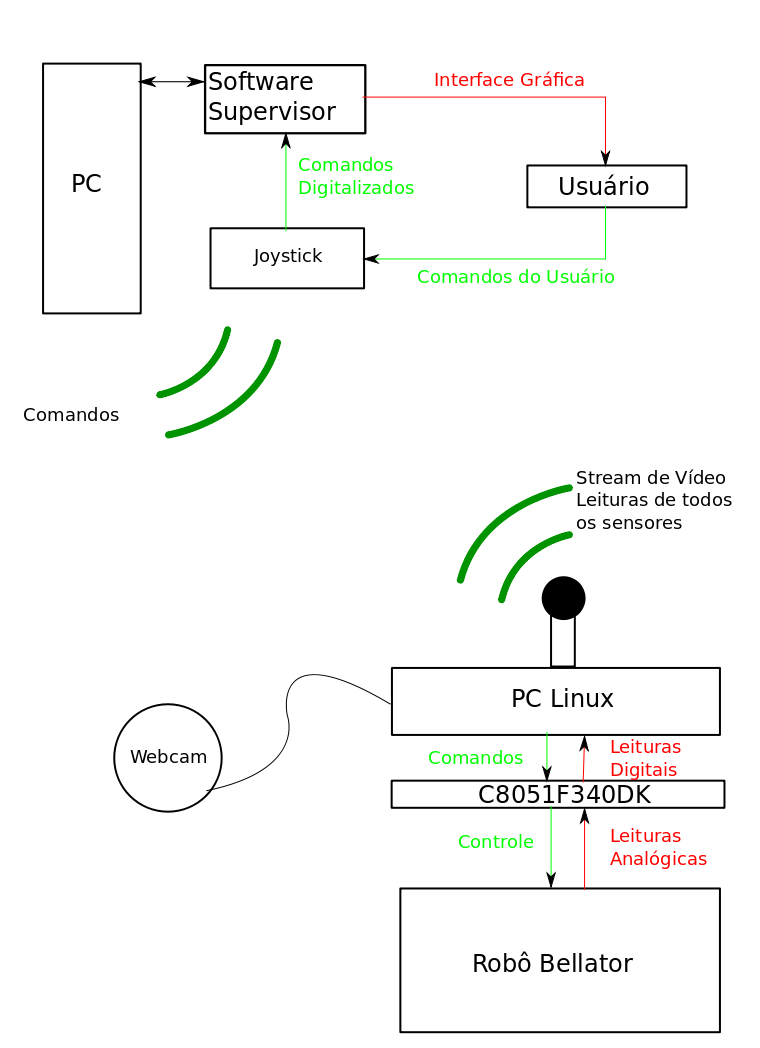
\includegraphics[width=0.8\textwidth]{./figs/diagsis.png}
	\caption[Diagrama original do Bellator]{Diagrama original do projeto Bellator, retirado da monografia do mesmo.}
	\fonte{\cite{BELLATOR}}
	\label{fig:diagsis}
\end{figure}

A partir da figura \ref{fig:diagsis}, o funcionamento do projeto Bellator pode ser explicado. A camada de baixo n�vel � composta pelo rob� Bellator, equipado com dois motores el�tricos Bosch FPG 12V, cinco sensores de dist�ncia ``2Y0A02F98"~ da Sharp, uma bateria Unybatt 12V-7,2 Amp�re hora, duas pontes H e a placa microcontrolada C8051F340, capaz de ler e converter leituras de tens�o anal�gicas dos sensores do rob� bem como produzir sinais de controle para os motores do rob�. Esta placa est� conectada � camada de alto n�vel, composta por um PC Embarcado VIA EPIA ME60000 Mini-ITX com sistema operacional Linux, atrav�s de uma conex�o serial. Utilizando-se de um protocolo de comunica��o, esse PC embarcado envia comandos de movimenta��o para a camada de baixo n�vel (conex�o serial) e recebe as leituras dos sensores obtidas pela camada de baixo n�vel. O PC embarcado tamb�m comunica-se com a camada supervis�ria para receber comandos de movimenta��o do usu�rio e enviar as leituras dos sensores para o mesmo (comunica��o sem fio). Al�m disso, o PC embarcado envia para a camada supervis�ria, tamb�m via comunica��o sem fio, um stream de v�deo gerado por uma webcam Genius iLook 316. Finalmente, o software supervisor remoto, executado em um PC com m�quina virtual Java, fornece as informa��es recebidas da camada de alto n�vel para o usu�rio, permitindo-o tomar decis�es sobre a locomo��o do rob�. O software tamb�m recebe comandos de movimenta��o do usu�rio, gerados em um Joystick do videogame Sony Playstation 2, enviando-os para a camada de alto n�vel pela mesma conex�o. Ao receber os comandos de movimenta��o, a camada de alto-n�vel simplesmente os repassa para a camada de baixo n�vel, respons�vel pela efetiva��o dos comandos, alterando os n�veis de PWM dos motores de acordo com os comandos recebidos.

O leitor pode observar que o projeto Bellator apresenta objetivos muito distintos do projeto ``Algoritmos de Navega��o Fuzzy: Uma An�lise Qualitativa". Assim, n�o ser� feita uma descri��o detalhada de todos os componentes do projeto Bellator, entretanto, pode-se consultar a refer�ncia \cite{BELLATOR} para mais informa��es. A seguir, ser� descrito como o rob� foi recebido pela equipe e quais componentes foram reaproveitados.

\subsection{Recebimento do Rob�}
\label{sec:recrobo}

O rob� Bellator foi entregue � equipe em Abril de 2011, em uma caixa, desmontado, juntamente com toda a documenta��o dispon�vel por m�dia digital. A caixa continha os seguintes itens:

\begin{itemize}
\item Chassi do rob� Bellator com dois motores Bosch FPG12V e pontes H acoplados;
\item Cinco sensores de dist�ncia ``2Y0A02F98"~ da Sharp;
\item Duas baterias Unybatt 12V-7,2 Amp�re hora;
\item Uma placa micro-controlada C8051F340;
\item Uma placa de roteamento, produzida pelo projeto Bellator;
\item Um PC Embarcado VIA EPIA ME60000 Mini-ITX.
\end{itemize}

O chassi do rob� e seus componentes acoplados s�o a base da plataforma rob�tica a ser utilizada pela equipe e s�o cr�ticas para a execu��o desse trabalho. Os sensores de dist�ncia s�o essenciais para a localiza��o de obst�culos, fornecendo informa��es cruciais para determina��o das a��es a serem tomadas. A placa microcontrolada tamb�m � um recurso cr�tico, pois � o componente respons�vel por todo o controle de baixo n�vel do rob� (acionamento dos motores, convers�o das leituras dos sensores, contagem dos pulsos dos encoders). As baterias s�o um recurso necess�rio e de f�cil aquisi��o, ao contr�rio dos outros componentes citados.

Alguns itens mencionados na se��o anterior, referentes ao projeto Bellator, n�o foram recebidos ou n�o ser�o utilizados nesse trabalho. A webcam e joystick n�o foram entregues pois n�o ser�o necess�rios, visto que um sistema de navega��o aut�nomo n�o � necess�rio o joystick e esse trabalho n�o abordar� navega��o atrav�s de imagem de v�deo. A placa de roteamento entregue ser� utilizada nos testes dos componentes, visto que � essencial para o funcionamento do rob�. Esta placa ser� reprojetada e reconstru�da. O PC embarcado foi entregue destitu�do de qualquer documenta��o. Al�m disso, como o novo objetivo do rob� n�o necessita de comunica��o sem fio e n�o utilizar� stream de v�deo, motivo principal para a utiliza��o deste PC no projeto Bellator~\cite{BELLATOR}, a equipe optou por descartar este recurso do projeto e utilizar outra placa mais simples e menor, que ser� descrita em detalhes na se��o \ref{chap:esprob}.

A documenta��o dispon�vel � equipe, produzida durante o projeto Bellator, descreve em detalhes os componentes de hardware dessa plataforma rob�tica, o software de controle supervis�rio e a camada de baixo n�vel, ou seja, o software da placa C8051F340~\cite{BELLATOR}. Essa documenta��o ser� utilizada como refer�ncia para o reaproveitamento do projeto Bellator nesse trabalho, com exce��o da documenta��o referente ao software de controle supervis�rio, que n�o ser� utilizado. O processo de reconstru��o e adapta��o da plataforma rob�tica � descrito em detalhes no cap�tulo \ref{chap:desenv}.

\subsection{Considera��es}
A possibilidade de reaproveitamento parcial do projeto Bellator e o recebimento desse material consistiram uma importante etapa nesse trabalho. A plataforma Bellator � uma op��o de recurso ao apoio do estudo qualitativo proposto nesse TCC.

%---------- Especifica��es do hardware do rob� ----------
\section{Especifica��es do Rob�}
\label{sec:esprob}

Esta se��o visa descrever a composi��o de \emph{hardware} do rob�
Bellator ap�s a reconstru��o e adequa��o do mesmo. Essa decri��o
inclui a apresenta��o dos sensores infravermelhos, enconders
�pticos, placa microcontrolada C8051F340DK, placa TS-7260, placa de roteamento e a apresenta��o do produto final, ou seja, o rob� montado.

\subsection{Sensor IR 2Y0A02F98}
\label{sec:sensores}
O sensor 2Y0A02F98 � um sensor anal�gico infravermelho e mede dist�ncias no intervalo de 20 a 150 cent�metros \cite{datasheetsensor}, sendo que os valores de tens�o de resposta do sensor seguem a curva mostrada na figura \ref{curva}. Como o valor de leitura � anal�gico, foi necess�rio que a placa C8051F340DK fosse programada para converter essa leitura em digital. O c�digo de convers�o est� de acordo com o projeto Bellator \cite{BELLATOR} e tamb�m efetua a transfer�ncia desses dados por comunica��o serial.

\begin{figure}[H]
  \centering
  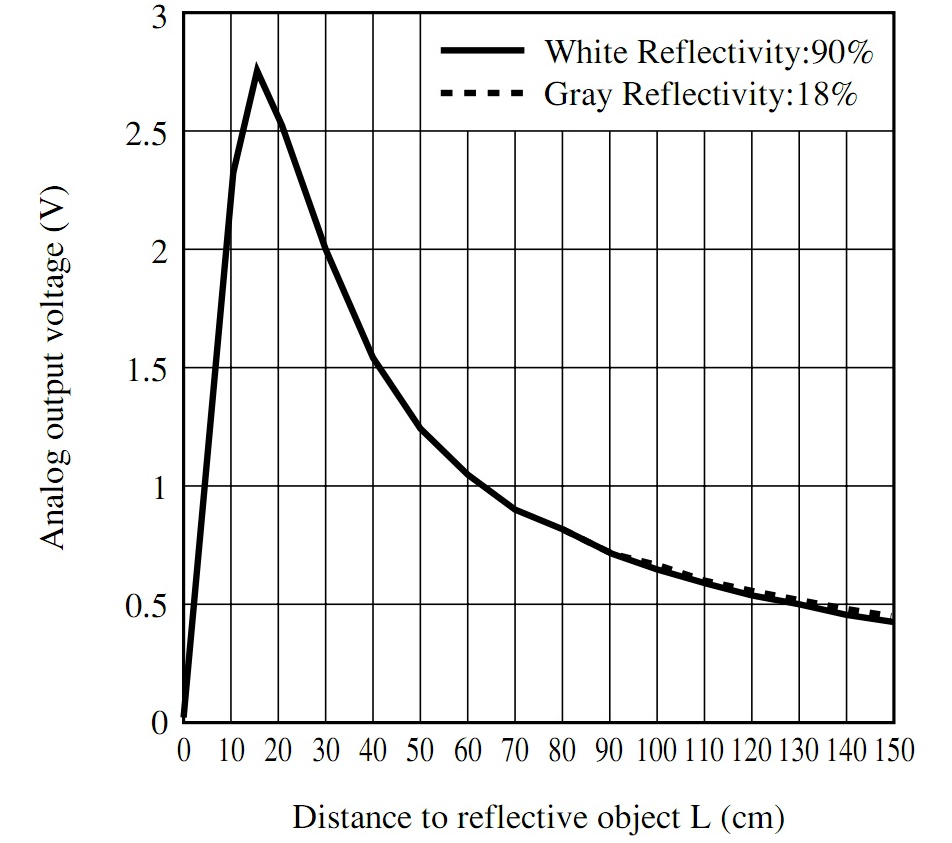
\includegraphics[width=0.5\textwidth]{./figs/curvaresp.png}
  \caption[Curva de resposta do sensor de dist�ncia]{Curva de resposta do sensor de dist�ncia.}
  \fonte{\cite{datasheetsensor}}
  \label{curva}
\end{figure}

O modelo � pouco influenciado pelas cores dos objetos refletidos, isso � devido ao m�todo de medi��o baseado em triangula��o \cite{datasheetsensor}. O sensor possui uma tens�o de alimenta��o recomendada na faixa de 4,5 a 5,5 V \cite{datasheetkit}. Como as baterias dispon�veis eram de 12 V, foi necess�ria utiliza��o de um regulador de tens�o. O c�lculo dos valores dos resistores foram baseados na equa��o \ref{eqRegulador} e o diagrama esquem�tico do regulador � mostrado na figura \ref{regulador}. Esse circuito comp�e uma das partes da placa de roteamento, conforme mostrado na se��o \ref{sec:espplacaroteamento}.

\begin{equation}
\label{eqRegulador}
V_{OUT} = 1,25V (1 + R_{2}/R_{1})
\end{equation}

\begin{figure}[H]
  \centering
  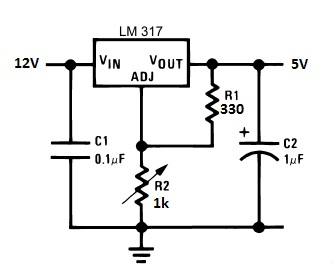
\includegraphics[width=0.5\textwidth]{./figs/regulador.jpg}
  \caption[Diagrama esquem�tico do regulador de tens�o dos sensores de dist�ncia]{Diagrama esquem�tico do regulador de tens�o dos sensores de dist�ncia.}
  \fonte{\cite{LM317}}
  \label{regulador}
\end{figure}

O modelo em quest�o � adequado ao projeto pois apresenta dimens�es compat�veis com o chassi do rob� e, como a finalidade desses sensores � auxiliar a navega��o do rob� em ambientes fechados, a faixa de resposta � suficiente para detec��o de objetos. Contudo, h� a possibilidade de, em projetos futuros, acrescentar outros tipos de sensores mais precisos voltados � medi��o de dist�ncias menores.

\subsection{Encoder �ptico HEDS-9700}
\label{sec:heds9700}
O \emph{encoder} �ptico HEDS-9700 � um circuito capaz de gerar uma onda quadrada � medida que um \emph{encoder} de quadratura � rotacionado \cite{HEDS9700}. A curva de resposta desse sensor � ilustrada na figura \ref{fig:HEDS-9700}. Nessa figura s�o ilustrados dois canais A e B, havendo um defasamento de $\phi$ entre os sinais. Nesse projeto, foi utilizado o sinal de apenas um dos canais, pois a informa��o desejada era simplesmente a contagem de pulsos gerada por cada encoder. O \emph{encoder} de quadratura utilizado na plataforma rob�tica est� fixado no eixo de cada roda e apresenta 1800 pulsos por volta. A placa C8051F340DK foi programada para contar esses pulsos e fornecer uma medida odom�trica para realimenta��o da velocidade. Essa programa��o � descrita na se��o \ref{sec:codmicro} e permite ajustar a velocidade das rodas de forma independente. Como a placa de roteamento do projeto de oficinas \cite{BELLATOR} n�o foi projetada para tratar o sinal deste \emph{encoder}, foi projetada uma nova vers�o dessa placa, descrita na se��o \ref{sec:espplacaroteamento}.

\begin{figure}[H]
  \centering
  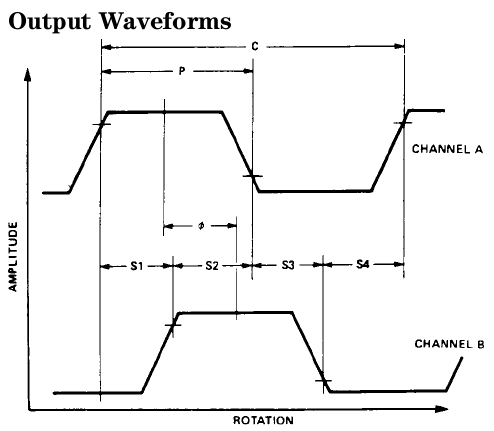
\includegraphics[width=0.5\textwidth]{./figs/HEDS-9700.png}
  \caption[Formas de onda de sa�da do \emph{encoder} �ptico]{Formas de onda de sa�da do encoder �ptico.}
  \label{fig:HEDS-9700}
  \fonte{\cite{HEDS9700}}
\end{figure}

\subsection{C8051F340DK}
\label{sec:C8051F340DK}

O C8051F340 � uma unidade microcontroladora (MCU) equipada com um n�cleo da fam�lia 8051 e v�rios dispositivos perif�ricos dispostos em uma placa de circuito impresso. As especifica��es dessa unidade foram retiradas do relat�rio do projeto Bellator \cite{BELLATOR}. O diagrama em blocos do kit � apresentado na figura \ref{dbloc}. A C8051F340 possui as seguintes caracter�sticas \cite{datasheetkit}:

\begin{itemize}
  \item Conversor ADC 10 bits de at� 200 ksps (amostras por segundo);
  \item Dois comparadores;
  \item \emph{Brown-out Reset} e \emph{Power-on Reset};
  \item Tens�o de Refer�ncia interna;
  \item Porta USB 2.0;
  \item Duas \emph{interfaces} seriais (UART) e uma \emph{interface} SPI;
  \item Fonte de Alimenta��o de 2.7 at� 5.25V regulada internamente;
  \item Micro-processador 8051 de at� 48 MIPS;
  \item 4352 Bytes de mem�ria RAM;
  \item 40 Portas de E/S;
  \item 4 temporizadores de 16 bits;
  \item Sele��o de \emph{clock} interno de alta ou baixa velocidade ou \emph{clock} externo.
\end{itemize}

\begin{figure}[H]
  \centering
  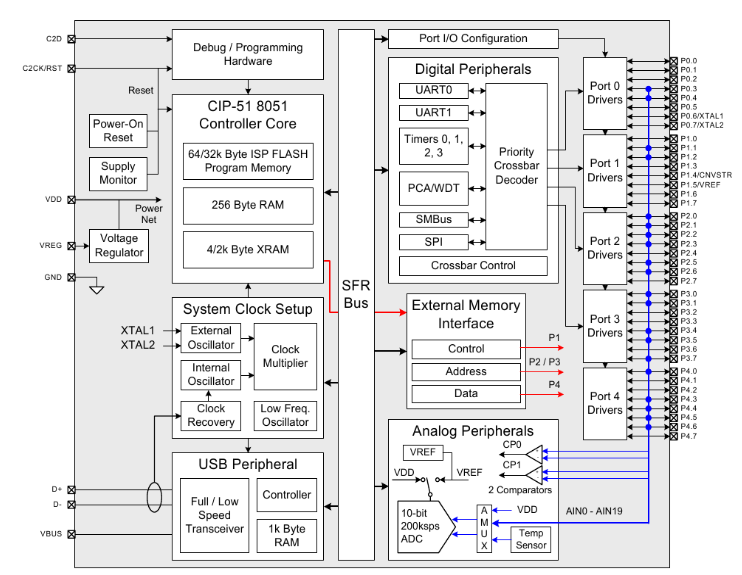
\includegraphics[width=0.8\textwidth]{./figs/dbloc.png}
  \caption[Diagrama em blocos do kit C8051F340DK]{Diagrama em blocos do kit C8051F340DK.}
  \fonte{\cite{datasheetkit}}
  \label{dbloc}
\end{figure}

\subsection{Placa TS-7260}
\label{sec:espts7260}

A placa TS-7260 � um sistema embarcado equipado com um processador ARM e sistema operacional Linux. O sistema possui perif�ricos para realiza��o de comunica��o serial, ethernet, usb, entre outros. A lista a seguir descreve os componentes relevantes para o projeto. Os dados, bem como a figura \ref{fotots}, foram retirados do \emph{datasheet} \cite{TS-7260}.

\begin{itemize}
  \item Processador ARM9 de 200MHz baseado no Cirrus EP9302
  \item 32MB de mem�ria NAND Flash
  \item 32MB de mem�ria SDRAM
  \item Consumo menor que 1 Watt mesmo em capacidade m�xima
  \item Porta Ethernet 10/100
  \item Duas portas USB 2.0
  \item Entrada de 4.5 a 20 Volts
  \item Dimens�es: 9.7 cm por 11.5cm
\end{itemize}

\begin{figure}[H]
  \centering
  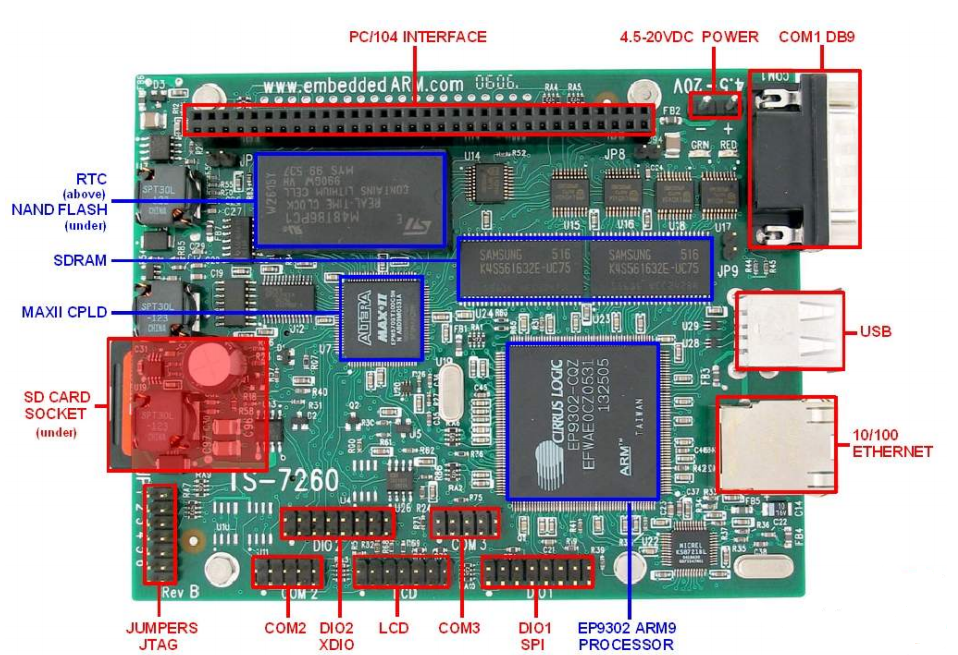
\includegraphics[width=0.8\textwidth]{./figs/fotots.png}
  \caption[Foto da placa TS-7260]{Foto da placa TS-7260.}
  \fonte{\cite{tsmanual}}
  \label{fotots}
\end{figure}

Mais informa��es sobre o sistema, bem como a documenta��o completa, est�o dispon�veis no manual da placa, dispon�vel nas refer�ncias bibliogr�ficas \cite{tsmanual}.

\subsection{Placa de Roteamento}
\label{sec:espplacaroteamento}

A placa de roteamento � um componente desenvolvido com base na placa dispon�vel do projeto Bellator \cite{BELLATOR}. Como a placa de roteamento recebida com o Bellator n�o tratava os sinais dos \emph{encoders} e estava constru�da de forma rudimentar, em uma placa universal, ela foi reprojetada e reconstru�da pela equipe. As especifica��es da placa de roteamento s�o:
\begin{itemize}
    \item Dimens�es: 5 x 9 cm;
    \item Trilhas de cobre de aproximadamente 1 mm;
    \item Regulador de tens�o LM317T: Entrada at� 40V, Sa�da 5,05V;
    \item \emph{Buffer} para PWM: 74LS244;
    \item Conectores para cabos \emph{flat}, PWM, Sensores e \emph{Encoders}.
\end{itemize}

O projeto da placa, m�todos de desenvolvimento, requisitos, entre outros ser�o descritos de forma detalhada na se��o \ref{sec:desroteamento}.

\subsection{Rob� Bellator}
\label{sec:robobellator}

O rob� Bellator, como mencionado na se��o \ref{sec:estpro}, foi reconstru�do e adaptado ao projeto. O rob� consiste de um chassi de 40 cm de largura por 50 cm de comprimento, duas rodas de tra��o e uma roda guia, conforme ilustrado na figura \ref{fig:dispsensor}. As rodas de tra��o est�o nas laterais da parte dianteira do rob� e possuem di�metro de 20 cm e largura de 4 cm. Ambas possuem o \emph{encoder} �ptico HEDS-9700, descrito na se��o \ref{sec:heds9700}, fixados nos respectivos eixos. A roda guia est� no centro da parte traseira do rob� e possui di�metro de aproximadamente 6 cent�metros e espessura de 2 cent�metros. Todas as rodas s�o da marca Schioppa e chassi do rob� permanece a 3 cm da superf�cie do solo. Com o objetivo de auxiliar a navega��o do rob� e fazer varreduras do ambiente, foram fixados cinco sensores do modelo 2Y0A02F98, descrito na se��o \ref{sec:sensores}, dispostos uniformemente nas laterais do chassi, conforme ilustra a figura \ref{fig:dispsensor}. Os outros componentes do rob� est�o listados a seguir:
\begin{itemize}
  \item[-] 2 Motores Bosch FPG 12V;
  \item[-] 2 Baterias Unybatt 12V-7,2 Amp�re-hora;
  \item[-] Duas pontes H L 298.
\end{itemize}

\begin{figure}[H]
  \centering
  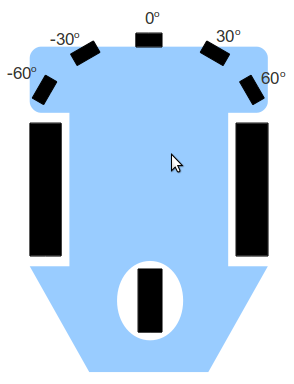
\includegraphics[width=0.3\textwidth]{./figs/dispsensor.png}
  \caption[Disposi��o dos sensores infravermelhos e rodas]{Disposi��o dos sensores infravermelhos e rodas.}
  \fonte{Autoria pr�pria}
  \label{fig:dispsensor}
\end{figure}

A plataforma transporta as placas do sistema microcontrolado C8051F340DK, descrito na se��o \ref{sec:C8051F340DK}, o sistema embarcado TS-7260, descrito na se��o \ref{sec:espts7260} e a placa de roteamento, descrita na se��o \ref{sec:espplacaroteamento}. O rob� montado pode ser visualizado na figura \ref{bellator}, que ilustra a disposi��o dos sensores infravermelhos, rodas, baterias e placas no chassi.

\begin{figure}[H]
  \centering
  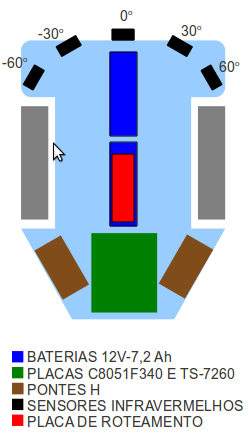
\includegraphics[width=0.3\textwidth]{./figs/bellator.png}
  \caption[Rob� Bellator montado]{Rob� Bellator montado.}
  \fonte{Autoria pr�pria}
  \label{bellator}
\end{figure}



\section{L�gica Fuzzy}
\label{sec:logfuzzy}
Esta se��o descreve os conceitos fundamentais utilizados pela equipe para o entendimento e implementa��o do algoritmo de navega��o fuzzy, descrito em detalhes na se��o \ref{sec:algfuzzy}.

\subsection{Conjuntos Fuzzy}

A teoria de conjuntos fuzzy foi elaborada inicialmente por Lofti Zadeh \cite{ZADEH}, visando explorar a possibilidade de criar um novo crit�rio de afilia��o � conjuntos. Na teoria cl�ssica de conjuntos, um elemento pode apenas pertencer ou n�o a um conjunto, sendo imposs�vel um n�vel de pertin�ncia parcial. J� em um conjunto fuzzy, isto torna-se poss�vel.
Um conjunto fuzzy pode ser definido por um conjunto de pares ordenados com o elemento e sua pertin�ncia ao conjunto fuzzy. Seja F um conjunto fuzzy e X um conjunto de objetos arbitr�rios, tem-se:

\begin{equation}
F=\{(x,f(x)),x\in X\}, f(x) = [0,1]
\end{equation}

Assim sendo, considere um conjunto ``A"~ simples que contenha tudo o que tem sabor doce. Neste conjunto uma barra de chocolate � doce da mesma forma que cana de a�ucar, visto que ambos pertencem ao conjunto, ou seja:
(barra de chocolate) $\in$ A e (cana de a�ucar) $\in$ A
Em um conjunto fuzzy B que contemple tudo o que tem sabor doce, torna-se poss�vel atribuir um n�vel de afilia��o ao conjunto atrav�s de uma fun��o de pertin�ncia f  permitindo dizer que, por exemplo, a cana de a�ucar � doce com n�vel de pertinencia 1, enquanto que a barra de chocolate � doce com n�vel de pertin�ncia 0.8, ou seja:\\*

\begin{center}
((cana de a�ucar),f(cana de a�ucar)) $\in$ B, f(cana de a�ucar) = 1\\*
((barra de chocolate),f(barra de chocolate)) $\in$ B, f(barra de chocolate) = 0.8\\*
\end{center}

Isto aproxima-se mais da forma como a cogni��o e intui��o humana funcionam, frequentemente utilizando palavras como ``mais", ``muito", ``pouco", entre outras, para definir graus de pertin�ncia a conjuntos de uma forma subjetiva.

\subsection{Vari�vel Lingu�stica}
\label{varling}

Uma aplica��o direta de conjuntos fuzzy � a defini��o de vari�veis lingu�sticas. \cite{PEDRYCZ}
Considerando que uma vari�vel \emph{x} pode assumir um valor qualquer dentro de um dado conjunto A, pode-se definir uma vari�vel lingu�stica como uma vari�vel cujo conjunto A de valores poss�veis � um conjunto de termos lingu�sticos, tais como: alto, baixo, curto, longo, entre outros. Pode-se estender este conceito associando cada termo lingu�stico poss�vel de uma vari�vel lingu�stica a um conjunto fuzzy.

Para entender esta defini��o, considere a vari�vel lingu�stica Temperatura (T) composta pelos termos lingu�sticos frio, morno e quente:
\begin{equation}
T = \{frio, morno, quente\}
\end{equation}
Considere tamb�m os seguintes conjuntos fuzzy:
\begin{equation}
	\begin{array}{lcl}
		F & = & \{(t,f(t)),t \in \mathbb{R}\} \\
		M & = & \{(t,m(t)),t \in \mathbb{R}\} \\
		Q & = & \{(t,q(t)),t \in \mathbb{R}\} \\
	\end{array}
\end{equation}
sendo \emph{\mbox{f(t), m(t) e q(t)}} fun��es de pertin�ncia, respectivamente, aos conjuntos fuzzy \emph{\mbox{F, M e Q}}, com valores de pertin�ncia pertencentes ao intervalo [0,1] e \emph{t} uma vari�vel representando a temperatura em um material qualquer. Considere ainda a associa��o dos conjuntos fuzzy \emph{\mbox{F, M e Q}} aos termos lingu�sticos frio, morno e quente, respectivamente. Neste cen�rio, um dado valor para a vari�vel \emph{t} pode ser traduzido em um valor equivalente para a vari�vel lingu�stica \emph{T}, dependendo apenas da defini��o das fun��es de pertin�ncia \emph{\mbox{f(t), m(t) e q(t)}}.

\begin{figure}[!htb]
	\centering
	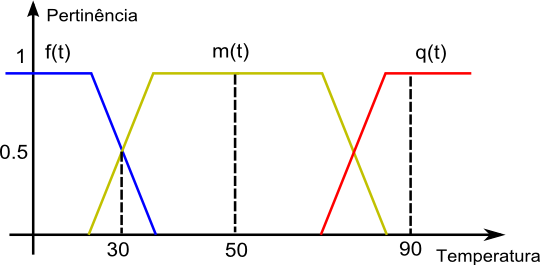
\includegraphics[width=0.8\textwidth]{./figs/fuzzygraph.png}
	\caption[Exemplo de Pertin�ncias Fuzzy]{Fun��es de Pertin�ncia f(t), m(t), q(t).}
	\label{fig:fuzzygraph}
\end{figure}

Se considerarmos, por exemplo, a defini��o gr�fica para as fun��es \emph{\mbox{f(t), m(t) e q(t)}} dada na figura \ref{fig:fuzzygraph}, e tr�s valores de temperatura, \emph{\mbox{t1 = 30, t2 = 50 e t3 = 90}}, temos que os valores correspondentes de temperatura para a vari�vel lingu�stica T s�o \mbox{T1 = (0.5 frio, 0.5 morno, 0.0 quente)}, \mbox{T2 = (0.0 frio, 1.0 morno, 0.0 quente)} e \mbox{T3 = (0.0 frio, 0.0 morno, 1.0 quente)}, respectivamente. Ou seja, informalmente, a temperatura t1 representa que o material est� ``meio frio"~ e ``meio morno"~, a temperatura t2 indica que est� ``morno"~ e a temperatura t3, por sua vez, ``quente"~. Este processo de convers�o para uma vari�vel lingu�stica � comumente chamado de ``fuzzifica��o".


\subsection{Controle Fuzzy}
\label{sec:fuzzycontrol}
Ap�s definidas as vari�veis lingu�sticas, conjuntos fuzzy e suas fun��es de pertin�ncia, descritas na se��o \ref{varling}, pode-se construir um controle fuzzy baseado em um conjunto de regras de infer�ncia.

Regras de infer�ncia sobre conjuntos fuzzy podem ser categorizadas como uma generaliza��o do \emph{modus ponens} bin�rio. Em l�gica bin�ria, dada regra ``se X ent�o Y", onde X e Y s�o vari�veis bin�rias, a partir do momento que a premissa, representada pela vari�vel X, assume valor l�gico verdadeiro, a conclus�o, dada por Y, � verdadeira tamb�m. Em l�gica fuzzy, o mesmo racioc�nio � valido, por�m X e Y s�o vari�veis lingu�sticas, e as regras de infer�ncia s�o definidas a partir dos valores que estas vari�veis lingu�sticas podem assumir, permitindo inclusive ativa��o parcial de regras de infer�ncia. Extendendo o exemplo das temperaturas, apresentado na se��o \ref{varling}, imagine que deseja-se controlar a velocidade de um \emph{cooler} de processador, de acordo com a temperatura que este se encontra, utilizando um controle fuzzy. As regras de infer�ncia para este controle podem ser, por exemplo:
\begin{center}
    Se \emph{morno} ent�o \emph{medio}\\*
    Se \emph{quente} ent�o \emph{forte}
\end{center}
Sendo ``medio"~ e ``forte"~ valores poss�veis da vari�vel lingu�stica Velocidade (V), que controla a velocidade do \emph{cooler}, com ``medio"~ correspondendo a fun��o de pertin�ncia vm e ``forte"~ correspondendo a vf, apresentados na figura \ref{fig:defuzzygraph}:

\begin{figure}[!htb]
	\centering
	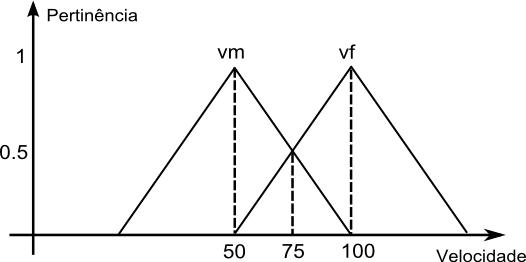
\includegraphics[width=0.8\textwidth]{./figs/defuzzygraph.png}
	\caption[Exemplo de Pertin�ncias Fuzzy - Defuzzifica��o]{Fun��es de Pertin�ncia vm e vf.}
	\label{fig:defuzzygraph}
\end{figure}

De acordo com estas regras de infer�ncia, se a temperatura \emph{fuzzificada} for inteiramente fria, nenhuma regra ser� ativada e a velocidade do \emph{cooler} ser� nula. Por�m, se a temperatura for maior que a m�nima necess�ria para come�ar a ser classificada como morna, haver� ativa��o integral ou parcial de uma ou ambas as regras de infer�ncia. Neste caso, � necess�rio determinar o grau de ativa��o de cada uma das regras e produzir uma sa�da que contemple estes graus de ativa��o, que � o processo inverso � \emph{fuzzifica��o}, a \emph{defuzzifica��o}. Um destes m�todos � a m�dia do m�ximo, que consiste da m�dia ponderada dos m�ximos de cada valor fuzzy de sa�da, com os pesos correspondendo �s ativa��es das regras de infer�ncia. Considerando novamente o exemplo do controle de velocidade de um \emph{cooler} e considerando que, em um determinado momento, a temperatura est� ``meio morno"~ e ``meio quente"~, ou seja, 0.5 de pertin�ncia � classe ``morno"~ e a classe ``quente"~, ambas as regras ser�o ativadas igualmente e a velocidade do \emph{cooler} ser�:
\begin{equation}
v = \frac{\left( 0.5*50 + 0.5*100 \right ) } {1} = 75
\end{equation}

\subsection{Considera��es}

O conceito de incerteza introduzido pela L�gica Fuzzy permite a modelagem de sistemas com problemas de decis�o cujas vari�veis s�o din�micas, reduzindo a influencia de ru�dos e possibilitando a constru��o de um sistema de infer�ncias an�logo � cogni��o humana. O problema de navega��o rob�tica � altamente din�mico, pois as decis�es s�o tomadas sob a influ�ncia de v�rios sensores simultaneamente, todos pass�veis de ru�do, e a abordagem Fuzzy � uma op��o plaus�vel para trat�-lo.

\section{Mapas Cognitivos Fuzzy}
\label{sec:fcm}
Esta se��o tem como objetivo explicar o que s�o mapas cognitivos fuzzy, tamb�m conhecidos como FCM (Fuzzy Cognitive Maps), abordando o conceito, a estrutura, as propriedades e vantagens desse modelo, apresentar os passos para contru��o de um FCM e apresentar exemplos, que descrevem o uso em situa��es reais.

O modelo FCM � abordado na tese de doutorado de \cite{FCMENDONCA}. Mapas cognitivos s�o diagramas que representam liga��es entre palavras, id�ias, tarefas ou outros itens ligados a um conceito central, dispostos radialmente, intuitivamente e de acordo com a import�ncia de cada conceito. Cren�as ou afirma��es a respeito de um dom�nio de conhecimento limitado s�o expressas por palavras ou express�es lingu�sticas interligadas por rela��es de causa e efeito, que possibilitam predizer as consequ�ncias que essa organiza��o implica ao universo representado. O mapa cognitivo fuzzy � gerado quando se incluem a essa estrutura incertezas atrav�s da l�gica Fuzzy.

\begin{figure}[!htb]
    \centering
    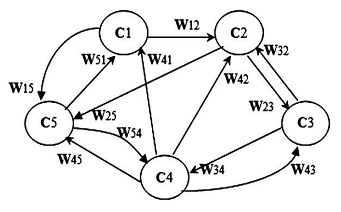
\includegraphics[width=0.5\textwidth]{./figs/fcm.png}
    \caption[Exemplo de um FCM]{Exemplo de um FCM (grafo).}
    \fonte{\cite{FCMENDONCA}}
    \label{fig:fcm}
\end{figure}

A estrutura de um FCM � um grafo direcionado, figura \ref{fig:fcm}, em que os valores num�ricos s�o vari�veis ou conjuntos fuzzy, os ``n�s"~ s�o conceitos lingu�sticos, representados por conjuntos fuzzy e cada ``n�"~ � associado a outros n�s atrav�s de conex�es (relacionamentos), a cada qual est� associado um peso num�rico, que representa a vari�vel fuzzy relacionada ao n�vel de causalidade entre os conceitos. De acordo com \cite{MENDONCA}, um FCM suporta diversos tipos de conceitos e relacionamentos:

\begin{itemize}
    \item Conceito de n�vel: Esse conceito pode pode ser representado por um valor absoluto;
    \item Conceito de varia��o: Esse tipo de conceito representa a varia��o de um valor no tempo;
    \item Conceitos de entradas: Esses conceitos recebem um valor de entrada e podem interagir com outros conceitos;
    \item Conceitos de sa�da ou de decis�o: Esses conceitos representam o resultado das infer�ncias do FCM e n�o interagem com outros conceitos;
    \item Rela��es causais: Essas conex�es representam as rela��es de causa e efeito entre os conceitos e s�o calculadas atrav�s da matriz de pesos (matriz W);
    \item Declara��es condicionais: Esses elementos s�o as rela��es causais expressas na forma de regras \emph{se-ent�o} e s�o atualizadas temporalmente.
\end{itemize}

Na figura \ref{fig:fcm}, os conceitos (C1 a C5) podem ser atualizados atrav�s da intera��o com outros conceitos por meio das rela��es causais ($w_{i,j}$) e com seu pr�prio valor. A matriz \ref{fcm-matrix} representa o peso das rela��es causais entre os conceitos e podem ser atualizados atrav�s da equa��o \ref{fcm-update}. Esta descreve a evolu��o do FCM, na qual j � o contador das itera��es, n � o n�mero de n�s do grafo, $W_{ji}$ � o peso do arco que conecta o conceito $C_j$ ao conceito $C_i$, $A_i$ e $A_i^{anterior}$ s�o o valor do conceito $C_i$ na itera��o atual e anterior, respectivamente, e a fun��o f \ref{sigmoide} � uma fun��o do tipo sigm�ide.

\begin{equation}\label{fcm-matrix}
    w_{i,j}=\left(
       \begin{array}{ccccc}
         0 & w_{12} & 0 & 0 & w_{15} \\
         0 & 0 & w_{23} & 0 & w_{25} \\
         0 & w_{32} & 0 & w_{34} & 0 \\
         w_{41} & 0 & w_{43} & 0 & w_{45} \\
         w_{51} & 0 & 0 & w_{54} & 0 \\
       \end{array}
     \right)
\end{equation}

\begin{equation}\label{fcm-update}
A_i=f(\sum_{\substack{j=1 \\ j\neq i}}^{n} A_j \times W_{ji})+A_i^{anterior}
\end{equation}

\begin{equation}\label{sigmoide}
f(x)=\frac{1} {1+e^{-\lambda x}}
\end{equation}

Em \cite{KOSKO}, s�o apresentados os seguintes passos para constru��o de um FCM cl�ssico:

\begin{itemize}
\item Passo 1 - Identifica��o dos conceitos e das suas interconex�es ou rela��es
determinando a natureza (positiva, negativa ou neutra) das rela��es causais entre
conceitos;
\item Passo 2 - Aquisi��o de dados iniciais, atrav�s de pondera��o de opini�o de
especialistas e ou an�lise do sistema de equa��es, quando se conhece o modelo
matem�tico;
\item Passo 3 - Apresenta��o dos dados referentes � opini�o dos diversos especialistas a
um sistema l�gico fuzzy que tem como sa�da os valores dos pesos do FCM;
\item Passo 4 - Tratamento da informa��o, adapta��o e ou otimiza��o do FCM
inicialmente proposto, ajustando suas respostas �s sa�das desejadas;
\item Passo 5 - Valida��o do FCM ajustado nas condi��es de opera��o do sistema ou
processo modelado.
\end{itemize}

Um FCM apresenta as propriedades de elasticidade e estabilidade, sendo que a elasticidade, ou auto organiza��o, � a capacidade de refor�ar ou enfraquecer o peso das rela��es causais e a estabilidade � a capacidade de o mapa evoluir, estabilizando-se em um ponto fixo ou ap�s um n�mero m�ximo de itera��es. Uma vantagem do FCM � a modularidade, a qual permite que um problema complexo seja representado por v�rios mapas modulares e outra vantagem � que os pesos das rela��es causais e dos conceitos podem ser obtidos via treinamento a partir dos dados hist�ricos do sistema ou atrav�s de um algoritmo adaptativo, que atualiza os pesos constantemente.

\begin{figure}[!htb]
    \centering
    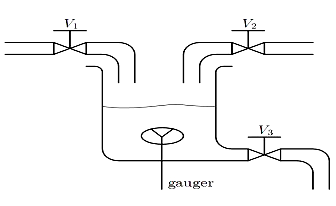
\includegraphics[width=0.5\textwidth]{./figs/fcm-exemplo-planta.png}
    \caption[Aplica��o do FCM em processo industrial]{Aplica��o do FCM em processo industrial.}
    \fonte{\cite{GROUMPOS}}
    \label{fig:fcm-exemplo-planta}
\end{figure}

Em \cite{GROUMPOS} os mapas cognitivos fuzzy s�o aplicados no controle de processos industriais. Um exemplo de aplica��o � mostrado na figura \ref{fig:fcm-exemplo-planta}, na qual � ilustrado um tanque com duas v�lvulas de entrada (V1 e V2) para diferentes tipos de l�quidos, um misturador, uma v�lvula de sa�da (V3) para o l�quido misturado e um medidor de massa espec�fica (G) que mede a quantidade de l�quido produzida. As v�lvulas V1 e V2 introduzem dois l�quidos diferentes. Durante a mistura, o medidor de massa espec�fica verifica quando o produto atingiu o ponto adequado e, desse modo, a v�lvula V3 � ativada e o produto da mistura � esvaziado. Analisando-se o problema, os seguintes conceitos podem ser definidos:

\begin{itemize}
\item Conceito 1: Volume de l�quido no tanque, o qual depende do estado das v�lvulas V1, V2 e V3;
\item Conceito 2: Estado da v�lvula 1 (fechada, aberta ou parcialmente aberta);
\item Conceito 3: Estado da v�lvula 2 (fechada, aberta ou parcialmente aberta);
\item Conceito 4: Estado da v�lvula 3 (fechada, aberta ou parcialmente aberta);
\item Conceito 5: Valor de massa espec�fica do l�quido medido pelo sensor G.
\end{itemize}

O controlador do processo deve manter as vari�veis V e G, sendo V o volume e G a massa especifica do produto no tanque, dentro das faixas de opera��o $[V_{min}, V_{max}]$ (equa��o \ref{lim-V}) e $[G_{min}, G_{max}]$ (equa��o \ref{lim-G}), respectivamente.

\begin{equation}\label{lim-V}
V_{min}<V<V_{max}
\end{equation}

\begin{equation}\label{lim-G}
G_{min}<G<G_{max}
\end{equation}

Interligando-se os conceitos atrav�s de rela��es de causa e efeito, o FCM da figura \ref{fig:fcm-exemplo-fcm} foi constru�do.

\begin{figure}[!htb]
    \centering
    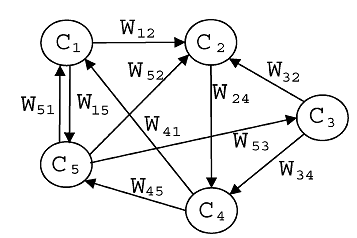
\includegraphics[width=0.5\textwidth]{./figs/fcm-exemplo-fcm.png}
    \caption[Mapa Cognitivo Fuzzy]{FCM do controlador.}
    \fonte{\cite{GROUMPOS}}
    \label{fig:fcm-exemplo-fcm}
\end{figure}

 Analisando-se o conhecimento dos especialistas, os pesos das rela��es s�o dados pelas inequa��es \ref{peso-1} a \ref{peso-8}.

\begin{equation}\label{peso-1}
-0,50<w_{12}<0,30
\end{equation}
\begin{equation}\label{peso-2}
-0,40<w_{13}<0,20
\end{equation}
\begin{equation}\label{peso-3}
0,20<w_{15}<0,40
\end{equation}
\begin{equation}\label{peso-4}
0,30<w_{21}<0,40
\end{equation}
\begin{equation}\label{peso-5}
0,40>w_{31}<0,50
\end{equation}
\begin{equation}\label{peso-6}
-1,0<w_{41}<0,80
\end{equation}
\begin{equation}\label{peso-7}
0,50<w_{52}<0,70
\end{equation}
\begin{equation}\label{peso-8}
0,30<w_{54}<0,40
\end{equation}

O controlador do processo foi executado e, ap�s a estabiliza��o, obtiveram-se os pesos da matriz \ref{W-matrix} e os valores dos conceitos da matriz \ref{A-matrix}. Os limites das equa��es \ref{lim-V} e \ref{lim-G} s�o reajustados para os valores correspondentes �s equa��es \ref{lim-V-adj} e \ref{lim-G-adj}, respectivamente, correspondendo ao ponto de opera��o desejado.

\begin{equation}\label{W-matrix}
    W^{inicial}=\left(
       \begin{array}{ccccc}
         0,00 & -0,40 & -0,25 & 0,00 & 0,30 \\
         0,36 & 0,00 & 0,00 & 0,00 & w0,00 \\
         0,45 & 0,00 & 0,00 & 0,00 & 0,00 \\
         -0,90 & 0,00 & 0,00 & 0,00 & 0,00 \\
         0,00 & 0,60 & 0,00 & 0,30 & 0,00 \\
       \end{array}
     \right)
\end{equation}

\begin{equation}\label{A-matrix}
    A^{inicial}=\left(
       \begin{array}{ccccc}
         0,10 & 0,45 & 0,39 & 0,04 & 0,01 \\
       \end{array}
     \right)
\end{equation}

\begin{equation}\label{lim-V-adj}
0,68<V<0,70
\end{equation}

\begin{equation}\label{lim-G-adj}
0,78<G<0,85
\end{equation}

Nesse exemplo, a estabiliza��o (ou sintonia) foi realizada atrav�s de tr�s m�todos: RNA (Rede Neural Artificial), AG (Algoritmo Gen�tico) e PSO (Particle Swarm Optimization ou Otimiza��o por Enxame de Part�culas).

Outra aplica��o � descrita no artigo \cite{MENDONCA}, na qual a abordagem FCM � empregada em navega��o rob�tica. Nesse artigo, um modelo de FCM novo � implementado para suportar as condi��es din�micas dos sistemas de navega��o, nas quais os valores das rela��es causais s�o modificados dinamicamente atrav�s da ocorr�ncia de eventos especiais. Os autores do artigo chamaram esse modelo de ED-FCM (Event-Driven Fuzzy Cognitive Map).

\begin{figure}[!htb]
    \centering
    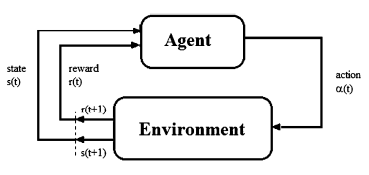
\includegraphics[width=0.5\textwidth]{./figs/reinforcement.png}
    \caption[Algoritmo de aprendizado por refor�o]{Algoritmo de aprendizado por refor�o.}
    \fonte{\cite{MENDONCA}}
    \label{fig:reinforcement-alg}
\end{figure}

O ajuste dos pesos das rela��es causais � efetuado por um algoritmo de aprendizado por refor�o, conforme ilustra a figura \ref{fig:reinforcement-alg}, e permite que o rob� (agente) aprenda diretamente atrav�s de sua intera��o com o ambiente. A cada instante de tempo t, o agente estabelece, por meio de seus sensores, um estado st e, de acordo com suas regras, determina uma a��o at a ser efetuada pelos atuadores. Essa a��o causa uma transi��o para o estado $s_{t+1}$ e o ambiente retorna uma medida de refor�o $r_{t+1}$, que pode ser uma recompensa (caso a a��o seja boa) ou uma puni��o (caso a a��o seja ruim).

\begin{figure}[!htb]
    \centering
    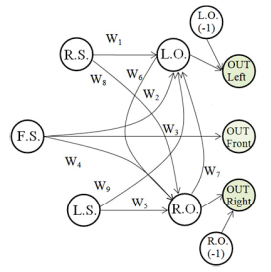
\includegraphics[width=0.5\textwidth]{./figs/fcm-robot.png}
    \caption[FCM do comportamento reativo do rob�]{FCM do comportamento reativo do rob�.}
    \fonte{\cite{MENDONCA}}
    \label{fig:fcm-robot}
\end{figure}

O FCM descreve o comportamento reativo do rob� (figura \ref{fig:fcm-robot}), no qual a leitura dos sensores de dist�ncia (esquerdo, frontal e direito) levam a uma a��o imediata que interfere no movimento. Os conceitos RS, FS e LS representam as leituras dos sensores, os conceitos LO e RO representam as decis�es de virar � esquerda ou virar � direita, respectivamente,  decis�es anteriores, representadas pelos conceitos LO(-1) e RO(-1), exercem influ�ncia sobre as decis�es atuais e a sa�da do algoritmo � representada pelos conceitos \emph{Out Left}, \emph{Out Front} e \emph{Out Right}. As rela��es causais do mapa s�o descritas na tabela \ref{tab:causal-relations} e as regras de a seguir determinam o comportamento do mapa:

\begin{enumerate}
\item SE a intensidade do sensor frontal (FS) for maior que um limiar m�dio ENT�O $W_{lim}$ aplicado para computar o relacionamento $w_3$ � o valor m�ximo de $WF_{max}$;
\item SE a intensidade do sensor frontal (FS) for menor que um limiar m�nimo ENT�O $W_{lim}$ aplicado para computar o relacionamento $w_3$ � o valor m�nimo de $WF_{min}$;
\item SE a intensidade do sensor direito (RS) for maior que um limiar m�dio ENT�O $W_{lim}$ aplicado para computar o relacionamento $w_1$ � o valor m�ximo de $WR_{max}$;
\item SE a intensidade do sensor direito (RS) for menor que um limiar m�nimo ENT�O $W_{lim}$ aplicado para computar o relacionamento $w_1$ � o valor m�nimo de $WR_{min}$;
\item SE a intensidade do sensor esquerdo (LS) for maior que um limiar m�dio ENT�O $W_{lim}$ aplicado para computar o relacionamento $w_5$ � o valor m�ximo de $WL_{max}$;
\item SE a intensidade do sensor direito (LS) for menor que um limiar m�nimo ENT�O $W_{lim}$ aplicado para computar o relacionamento $w_5$ � o valor m�nimo de $WL_{min}$.
\end{enumerate}

\begin{table}[htb!]
	\centering
	\caption[Rela��es causais do controlador do rob�]{Rela��es causais do controlador do rob�.}		
	\begin{tabular}[!htb]{ l l l l }
	  \hline
	  Rela��o causal & Descri��o & Efeito & Intensidade \\
	  \hline
	  $w_1$ & Sensor direito (RS) influencia a sa�da esquerda (LO) & Positivo & Forte \\
	  $w_2$ & Sensor frontal (FS) influencia a sa�da esquerda (LO) & Positivo & M�dio \\
	  $w_3$ & Sensor frontal (FS) influencia a sa�da frontal (FO) & Positivo & Forte \\
	  $w_4$ & Sensor frontal (FS) influencia a sa�da direita (RO) & Positivo & M�dio \\
	  $w_5$ & Sensor esquerdo (LS) influencia a sa�da direita (RO) & Positivo & Forte \\
	  $w_6$ & Sensor esquerdo (LS) influencia a sa�da direita (RO) & Negativo & Fraco \\
	  $w_7$ & Sensor direito (RS) influencia a sa�da esquerda (LO) & Negativo & Fraco \\
	  $w_8$ & Sensor direito (RS) influencia a sa�da direita (RO) & Negativo & Fraco \\
	  $w_9$ & Sensor esquerdo (LS) influencia a sa�da esquerda (LO) & Negativo & Fraco \\
	  \hline  	
	\end{tabular}
	\fonte{\cite{MENDONCA}}
	\label{tab:causal-relations}
\end{table}

Essas regras determinam a pol�tica de mudan�a de estados do mapa e os pesos dos relacionamentos s�o respons�veis pelas decis�es de o rob� virar � esquerda, acelerar ou virar � direita. Nesse contexto, o valor atual desses pesos depende da diferen�a entre os valores anteriores e o valor m�ximo admiss�vel ponderado por um fator $\gamma$ . O incremento dos pesos tamb�m leva em conta o valor da recompensa ou punic�o (r) e de um fator de aprendizagem $\alpha$ , os quais est�o associados ao algoritmo de aprendizado por refor�o escolhido, equa��o \ref{q-learning}.

\begin{equation}\label{q-learning}
w_i(k)=w_i(k-1)+\alpha \times [r+\gamma \times W_{lim}-w_i(k-1)]
\end{equation}

Por fim, nesse artigo, s�o descritos os resultados nos quais o rob�, em simula��o, foi capaz de desviar obst�culos � direita e � esquerda do mesmo ao longo da trajet�ria.

\subsection{Considera��es}
O FCM representa um problema em termos de conceitos e rela��es causais, podendo ser empregado em controladores de processos industriais ou no controle de rob�s aut�nomos. O problema do desvio de obst�culos em navega��o rob�tica p�de ser modelado, conforme o exemplo apresentado (figura \ref{fig:fcm-robot}), atrav�s de tr�s conceitos de entrada (RS, FS e LS), dois conceitos de decis�o (RO e LO), tr�s conceitos de sa�da (Right Out, Front Out e Left Out), rela��es causais, regras \emph{SE-ENT�O} e um algoritmo de aprendizado. O controlador proposto permitiu que o rob� desviasse obst�culos reagindo � leitura de sensores que medem a dist�ncia de objetos posicionados � esquerda e � direita do mesmo, concluindo-se que a abordagem FCM � adequada para esse trabalho.



%---------- Segundo Capitulo ----------
\chapter{Desenvolvimento}
\label{chap:desenv}

Este cap�tulo cont�m, em detalhes, o desenvolvimento do trabalho realizado pela equipe, dividido nas seguintes se��es:
\begin{itemize}
    \item[-] Reconstru��o da Plataforma Rob�tica Bellator: Todos os passos realizados para reconstruir e adaptar a plataforma rob�tica para utiliza��o no projeto e em trabalhos futuros.
    \item[-] Algoritmos de Navega��o: Detalha a implementa��o dos algoritmos de navega��o fuzzy e FCM, de acordo com as respectivas revis�es bibliogr�ficas apresentadas no cap�tulo \ref{chap:fundteor}.
    \item[-] Testes e An�lise de Resultados: Apresenta a metodologia e elabora��o dos testes dos algoritmos e a an�lise dos resultados obtidos para ambos os algoritmos de navega��o.
    \item[-] Considera��es: Conclus�o do cap�tulo e considera��es sobre o desenvolvimento do projeto.
\end{itemize}

\section{Reconstru��o da Plataforma Rob�tica Bellator}
\label{sec:recplat}
A reconstru��o e adapta��o da plataforma rob�tica Bellator, bem como a documenta��o da mesma para facilitar utiliza��o em trabalhos futuros, � um objetivo deste trabalho de conclus�o de curso e, portanto, esta se��o ir� descrever de forma detalhada todos os passos realizados pela equipe nesse processo de reconstru��o, incluindo os testes dos componentes recebidos no in�cio do projeto, elabora��o e instala��o de novos componentes de hardware para o rob� e documenta��o de componentes de software necess�rios para o funcionamento da plataforma rob�tica e para possibilitar a execu��o aut�noma de algoritmos de navega��o na mesma.

\subsection{Teste dos Componentes}
\label{sec:testecomp}

Ap�s o recebimento do rob�, foram realizados testes para garantir a funcionalidade dos componentes recebidos, j� que o rob�
estava com suas pe�as empilhadas numa caixa e n�o era poss�vel confiar no funcionamento adequado de nenhum dos componentes, al�m de que a falha de alguns componentes implicaria na impossibilidade de continuar o projeto ou em atrasos significativos. Estes testes tamb�m foram necess�rios para determinar de forma mais precisa o que poderia ser reaproveitado do projeto Bellator. De acordo com a documenta��o do projeto Bellator~\cite{BELLATOR}, o rob� deveria ser capaz de, se montado conforme as instru��es na mesma, funcionar como um sistema controlado remotamente. Como o objetivo deste projeto n�o envolve controlar
o rob� remotamente, foi testada apenas a camada de baixo n�vel.

O primeiro passo da etapa de testes foi verificar o funcionamento da placa C8051F340, pe�a fundamental para o desenvolvimento do projeto, que apresentou o funcionamento adequado, gerando os PWMs dos motores conforme necess�rio (visualizados no oscilosc�pio), e realizando a leitura dos sensores e convers�o A/D conforme esperado. Em seguida, foram iniciados os testes utilizando a placa de roteamento j� existente, que apresentou defeito. Ap�s alguns testes, foi constatado que a placa havia sido desconfigurada, v�rias soldas foram removidas, o circuito em si estava alterado. Ent�o, a equipe reorganizou a placa, realizou novos testes, mas n�o obteve sucesso. Foi ent�o verificado que
o regulador de tens�o n�o estava funcionando. Este foi substitu�do e a placa finalmente funcionou conforme esperado.

Com a placa de roteamento antiga funcionando, foi poss�vel realizar o teste dos motores, utilizando os PWMs gerados pelo
microcontrolador C8051F340 (entrada do buffer da placa de roteamento). Nesse teste, n�o ocorreram problemas, os motores funcionaram conforme esperado.

Das duas baterias inicialmente dispon�veis, uma n�o estava funcionando conforme a especifica��o, o que levou a equipe
a adquirir uma nova bateria 12V para reposi��o da bateria danificada.

Com todos os componentes acima citados testados, o que faltava para completar os testes da camada de baixo n�vel era apenas
o teste dos encoders. Esta etapa foi uma das mais dif�ceis, pois a equipe n�o tinha informa��o nem do modelo do encoder.
Depois de muito procurar, foi encontrado um datasheet de um encoder equivalente ao presente no rob�, datasheet este que foi fundamental para determinar como alimentar e testar o encoder. Em posse da informa��o de como usar o encoder, o teste foi realizado tanto para o encoder esquerdo como o direito. O encoder direito funcionou normalmente, por�m o esquerdo n�o. Ent�o, a equipe percebeu que a solda dos fios do encoder n�o estava boa. Ap�s refazer as soldas, o encoder esquerdo foi testado
novamente e funcionou.

Tendo realizado os testes dos componentes mais cr�ticos, o passo seguinte foi tentar utilizar o PC Embarcado VIA EPIA ME6000.
Ap�s muitas tentativas falhas e busca por informa��es sem resultados, a equipe optou por n�o utilizar este componente, j� que
sua documenta��o era escassa e o tempo perdido na tentativa de utiliz�-la j� estava acima do planejado (praticamente um m�s
foi gasto em tentativas frustradas). O PC Embarcado foi substitu�do pela placa TS-7260, que possui uma documenta��o muito
melhor, poder de processamento superior, e funcionou nos primeiros testes. Esta substitui��o n�o gerou custos para o projeto,
pois a placa TS-7260 j� havia sido adquirida para um projeto anterior e n�o estava sendo utilizada,
e foi ent�o disponibilizada � equipe pelo professor orientador Dr. Jo�o Alberto Fabro.

\subsection{Levantamento da curva dos sensores}
\label{sec:curvasensores}
Esta se��o apresenta como foi levantada a curva dos sensores, ponto fundamental para utilizar os
dados de convers�o, transformando-os para a dist�ncia em cent�metros, que ent�o pode ser passada
aos algoritmos de navega��o.

Primeiramente, foi montada uma tabela, contendo os valores de convers�o para cada dist�ncia, de 5
em 5cm, come�ando em 15cm at� 115cm, totalizando 21 medidas. Os valores obtidos est�o na tabela a
seguir:

\begin{table}[H]
\centering
\caption[Valores de convers�o dos sensores x dist�ncia]{Valores de convers�o dos sensores x dist�ncia}
\begin{tabular}{l l}
\hline
Valor da convers�o & Dist�ncia (cm) \\
\hline
207 & 15 \\
191 & 20 \\
173 & 25 \\
150 & 30 \\
134 & 35 \\
120 & 40 \\
110 & 45 \\
100 & 50 \\
91 & 55 \\
86 & 60 \\
81 & 65 \\
75 & 70 \\
71 & 75 \\
68 & 80 \\
66 & 85 \\
65 & 90 \\
62 & 95 \\
59 & 100 \\
56 & 105 \\
54 & 110 \\
50 & 115 \\
\hline

\end{tabular}
\label{tab:curvasensores}
\end{table}

A partir destes valores, foi realizada uma interpola��o polinomial para obten��o da equa��o aproximada
da curva. O grau do polin�mio interpolador escolhido foi o de grau 4, que aproximou\-se bem da curva
real (medida), conforme � poss�vel visualizar na figura~\ref{fig:curvasensores}, onde o eixo das abscissas
cont�m os valores de convers�o, e o eixo das ordenadas a dist�ncia correspondente. Segue a equa��o 
da interpola��o polinomial:

\begin{equation}
y = 3.6404 \cdot 10^{-7} x^4 - 2.4435 \cdot 10^{-4} x^3 + 6.0732 \cdot 10^{-2} x^2 - 6.8962x + 339.361
\end{equation}

\begin{figure}[H]
\centering
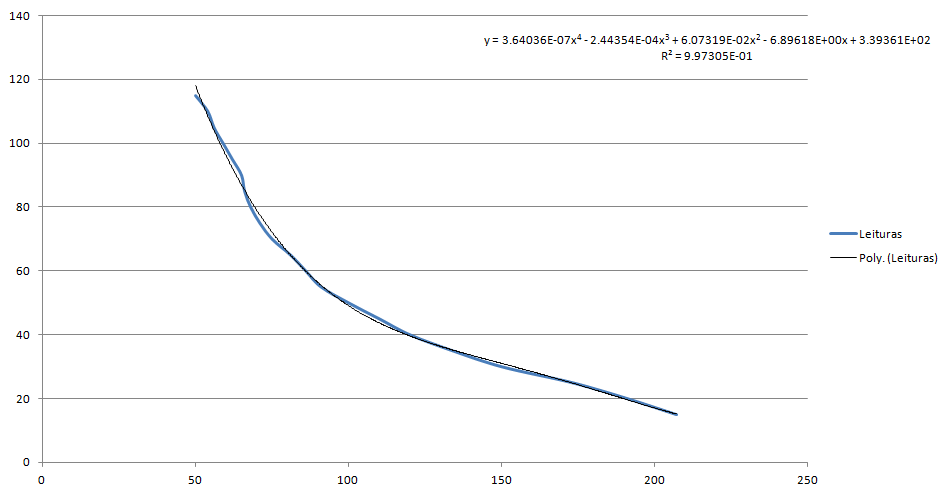
\includegraphics[width=0.95\textwidth]{./figs/curvaresp_poli.png}
\caption[Curva real dos sensores e interpola��o polinomial]{Curva real dos sensores e interpola��o polinomial}
\fonte{Autoria pr�pria}
\label{fig:curvasensores}
\end{figure}

Com esta equa��o, bastou iterar pelos valores \emph{x} poss�veis de convers�o (0 a 255, pois a convers�o
anal�gica/digital usa 8 bits) e montar a tabela para acessar com os valores de convers�o e obter
a dist�ncia em cent�metros. Esta tabela que mapeia os valores da convers�o para a dist�ncia em cent�metros
foi inserida no c�digo da placa TS-7260, que ser� explicado em detalhes na se��o~\ref{sec:softwarets}.

\subsection{C�digo do microcontrolador C8051F340}
\label{sec:codmicro}
Esta se��o apresentar� as fun��es do c�digo do microcontrolador, quais fun��es foram aproveitadas
do projeto Bellator, quais foram modificadas e quais foram implementadas por completo.

O c�digo que executa no microcontrolador tem diversas funcionalidades fundamentais do rob�, sendo elas:
leitura dos sensores de dist�ncia e convers�o anal�gica/digital dos sinais dos mesmos, gera��o dos
PWMs para ambos os motores, contagem dos pulsos dos encoders, recep��o e envio de mensagens atrav�s
da conex�o serial.

A �nica parte que foi implementada do zero neste projeto foi o tratamento dos sinais dos encoders (para obter
informa��es de odometria), informa��es estas essenciais para a execu��o dos algoritmos e consequente
navega��o aut�noma. O c�digo do projeto Bellator~\cite{BELLATOR} n�o continha o tratamento
dos sinais dos encoders (os encoders n�o haviam sido nem utilizados no projeto Bellator). Portanto,
foi necess�rio alterar o c�digo do microcontrolador para tratar os sinais
dos encoders e enviar informa��es de odometria. Para tal tarefa, foram utilizadas duas interrup��es
externas da placa C8051F340 (uma para cada encoder). Nestas interrup��es, cada pulso do encoder �
contado (obviamente cada encoder possui seu contador separadamente). A informa��o de contagem �
ent�o enviada atrav�s da comunica��o serial com a placa TS-7260 quando requerida pela mesma.
Os encoders est�o conectados � placa de roteamento, devido � necessidade de amplifica��o de seus
sinais para utiliza��o no microcontrolador. Na placa de roteamento, os sinais dos encoders s�o
amplificados em um amplificador operacional LM324~\cite{LM324}, e o sinal amplificado � ent�o conectado
ao Port 0 do microcontrolador.

A gera��o dos PWMs foi mantida como estava no projeto Bellator~\cite{BELLATOR}, com 76 n�veis poss�veis de PWM.
Os PWMs gerados s�o disponibilizados no Port 1 do microcontrolador, que � ent�o conectado � placa de
roteamento, onde os PWMs s�o utilizados como entrada para um buffer 74LS244~\cite{74LS244}, cujas sa�das
s�o utilizadas como PWM para as pontes H dos motores.

A leitura dos sensores de dist�ncia, que � realizada atrav�s de uma varredura (ao fim de cada convers�o,
o pr�ximo sensor � selecionado para convers�o), teve seu per�odo (este per�odo inclui a convers�o
de todas as leituras) alterado (de 1s para 50ms). Esta mudan�a foi necess�ria para permitir que
dados mais recentes sejam enviados ao rob�, para este poder reagir de forma mais adequada ao ambiente.
Os sensores est�o conectados � placa de roteamento, onde seus sinais de leitura s�o roteados para o
Port 2 do microcontrolador, que, por sua vez, realiza as convers�es A/D. Os valores obtidos s�o
simplesmente a convers�o do sinal de anal�gico para digital. Estes valores s�o enviados para a placa TS-7260
quando requeridos pela mesma, e somente na TS-7260 cada valor � utilizado para consultar a tabela, obtida
de acordo com o que foi descrito na se��o~\ref{sec:curvasensores}, mapeando o valor da convers�o
para a dist�ncia em cent�metros.

A parte de recep��o e envio de mensagens do c�digo do microcontrolador foi vastamente alterada,
para adequa��o ao protocolo descrito na se��o seguinte.



\subsection{Protocolo de comunica��o}
Esta se��o tem como objetivo explicar como funciona o protocolo de comunica��o, que foi desenvolvido
para padronizar a troca de mensagens com o microcontrolador C8051F340.

O protocolo de comunica��o nada mais � do que um arquivo que define quais s�o os bytes para cada tipo
de mensagem. Todas as mensagens, sejam elas recebidas ou enviadas pelo C8051F340, possuem o byte \emph{END\_CMD}
para sinalizar o fim de um comando/mensagem. As mensagens reconhecidas pelo microcontrolador C8051F340 s�o as seguintes:

\begin{itemize}
	\item \textbf{SYNC END\_CMD}: quando o microcontrolador C8051F340 recebe esta mensagem, responde
com as leituras mais recentes de cada sensor de dist�ncia, em seguida as leituras dos encoders;
	\item \textbf{LEFT\_WHEEL valor END\_CMD}: ao receber este comando, o microcontrolador utiliza o valor
para definir o n�vel de PWM para a roda esquerda do rob�. valor � representado por apenas um byte,
onde o bit mais significativo indica o sentido de rota��o da roda e os restantes a intensidade do PWM;
	\item \textbf{RIGHT\_WHEEL valor END\_CMD}: funcionamento id�ntico ao comando LEFT\_WHEEL, mas para a roda direita.
\end{itemize}

As mensagens enviadas pelo microcontrolador C8051F340 s�o apenas as respostas do comando SYNC:

\begin{itemize}
	\item \textbf{OPTICAL\_SENSOR\_[0-5] valor END\_CMD}: representa a leitura de cada sensor, onde
valor � um byte, cuja faixa de varia��o � [0, 255].
	\item \textbf{ENCODER valor\_high valor\_low END\_CMD}: representa a leitura de cada encoder,
valor\_high e valor\_low juntos formam um inteiro de 16 bits que cont�m o valor da contagem do encoder.
\end{itemize}

Esta se��o definiu o funcionamento do protocolo de comunica��o com o microcontrolador C8051F340,
para mais detalhes, basta consultar o arquivo do protocolo  (protocolo.h), onde os valores s�o definidos,
ou o c�digo do microcontrolador C8051F340, que define como as mensagens s�o interpretadas. O c�digo
da placa TS-7260 (tslogic.cpp), que cont�m as mensagens enviadas para a C8051F340, ser� explicado
em detalhes na se��o~\ref{sec:ts}.

\subsection{Placa de Roteamento}
\label{sec:desroteamento}

A placa de roteamento � um componente fundamental do projeto, respons�vel por realizar a interliga��o entre a placa C8051F340 e os componentes de hardware do rob�. A equipe constatou a necessidade deste componente devido aos seguintes fatores:

\begin{itemize}
    \item[-] Necessidade de alimenta��o dedicada para alguns componentes
    \item[-] Necessidade de tratamento dos sinais dos encoders
    \item[-] Roteamento das leituras de cada sensor para o pino I/O correto da C8051F340
    \item[-] Necessidade de um buffer para o PWM
    \item[-] Melhor organiza��o do rob�
\end{itemize}

Como descrito nas especifica��es do rob� (\ref{chap:esprob}), o rob� Bellator possui, dentre outros componentes, cinco sensores, dois encoders e duas pontes H. Os cinco sensores e dois encoders necessitam de alimenta��o de aproximadamente 5 Volts para opera��o. Os encoders produzem um sinal que precisa ser amplificado antes da utiliza��o, e as duas pontes H necessitam de um sinal de PWM de baixa imped�ncia. Al�m disso, o consumo de corrente total destes componentes ultrapassa a capacidade de fornecimento de corrente da C8051F340. Medi��es durante os testes com os componentes foram realizadas, e foi constatado que cada sensor de dist�ncia utiliza cerca de 30mA de corrente, enquanto os encoders utilizam 20mA cada, totalizando quase 200mA para estes componentes.

Por fim, a dificuldade de conectar, de forma pr�tica, todos os componentes do rob� com a C8051F340 bem como a quantidade excessiva de fios resultante fez com que a equipe conclu�sse que a placa de roteamento � indispens�vel.

De acordo com os fatores descritos, a equipe construiu uma lista de requisitos para a placa de roteamento:

\begin{itemize}
    \item[-] Fornecer alimenta��o de aproximadamente 5 Volts DC
    \item[-] Capacidade de corrente suficiente %Atualizar com valores!
    \item[-] Conectores pr�ticos para interface com a C8051F340 e o resto do rob�
    \item[-] Fornecer um buffer para o sinal de PWM
    \item[-] Fornecer amplifica��o para o sinal do encoder
\end{itemize}

Ap�s a an�lise dos requisitos, a equipe iniciou o desenvolvimento de uma placa de circuito impresso para atender a todos os requisitos. A necessidade de uma alimenta��o de 5 Volts tornou essencial a utiliza��o de um regulador de tens�o, o LM317, que era o mesmo utilizado na vers�o antiga da placa, e suporta corrente de at� 1.5A, valor suficiente para alimentar os componentes da placa. O buffer para o sinal de PWM foi feito atrav�s do CI 74LS244N e a amplifica��o dos sinais dos Encoders utilizando-se um amplificador operacional LM324N. O restante da placa consiste de pinos para conectar cabos flat, para a intera��o com a C8051F340, bem como pinos para conectores do hardware do rob� Bellator. O diagrama esquem�tico de tal placa foi produzido com o aux�lio do software Eagle e o resultado pode ser visualizado a seguir.

\begin{figure}[H]
  \centering
  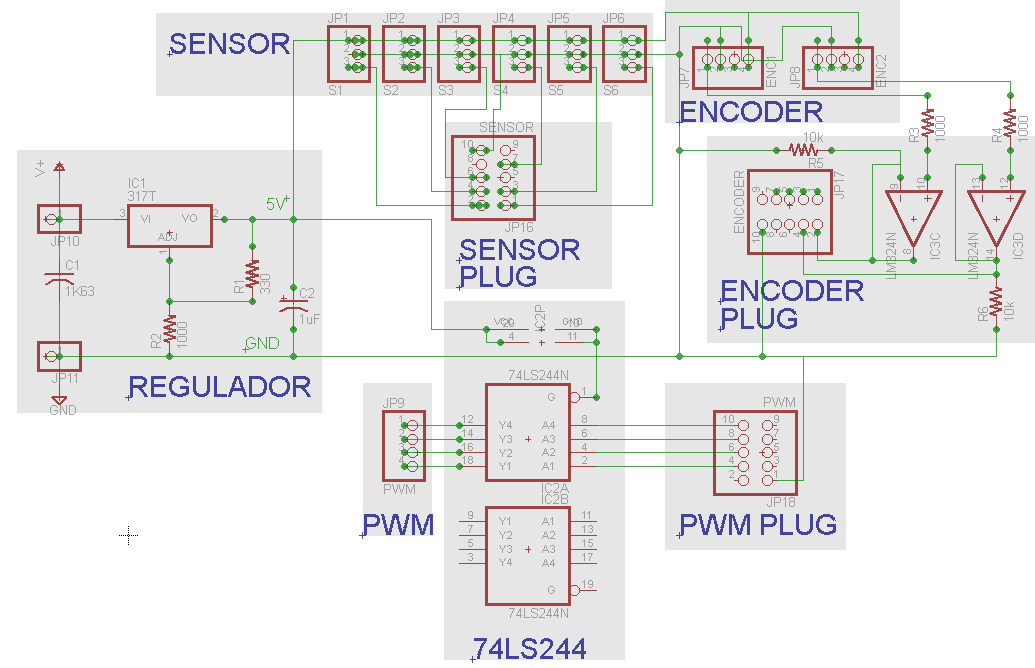
\includegraphics[width=0.8\textwidth]{./figs/roteamento_sch.png}
  \caption[Diagrama esquem�tico da placa de roteamento.]
  {Diagrama esquem�tico da placa de roteamento.}
  \label{fig:roteamento_sch}
\end{figure}

De posse do diagrama esquem�tico apresentado na figura \ref{fig:roteamento_sch} a equipe realizou o roteamento de uma placa de circuito impresso que atenda ao mesmo diagrama esquem�tico, tamb�m utilizando o software Eagle.

\begin{figure}[H]
  \centering
  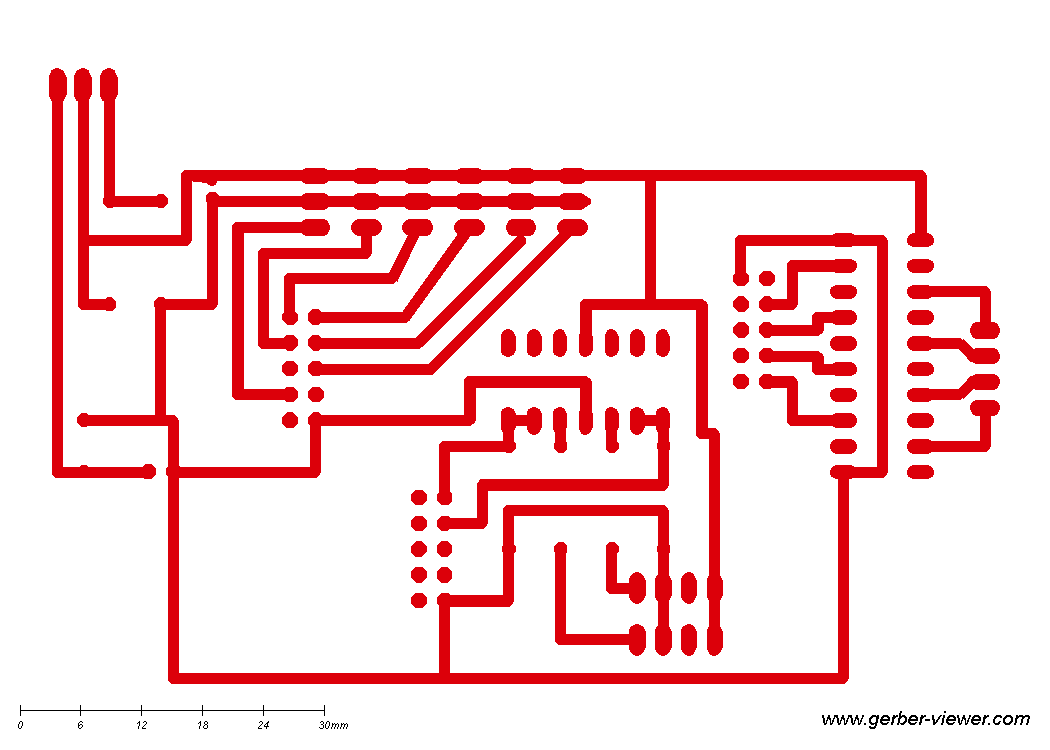
\includegraphics[width=0.8\textwidth]{./figs/roteamento_brd.png}
  \caption[Roteamento final produzido pela equipe.]
  {Roteamento final produzido pela equipe.}
  \label{fig:roteamento_brd}
\end{figure}

A placa de roteamento foi confeccionada manualmente em uma placa de circuito impresso. O desenho da placa foi impresso em uma folha de transpar�ncia A4 e utilzando-se uma impressora � laser. Esse desenho foi passado da traspar�ncia para a placa com o aux�lio de um ferro de passar roupa e a placa foi corro�da usando-se o percloreto de ferro. A placa foi perfurada com broca e perfurador de placa e os componentes eletr�nicos foram soldados com ferro de solda, estanho e pasta de solda. A figura \ref{fig:confeccao} ilustra o processo de confecc��o da placa.

\begin{figure}[H]
  \centering
  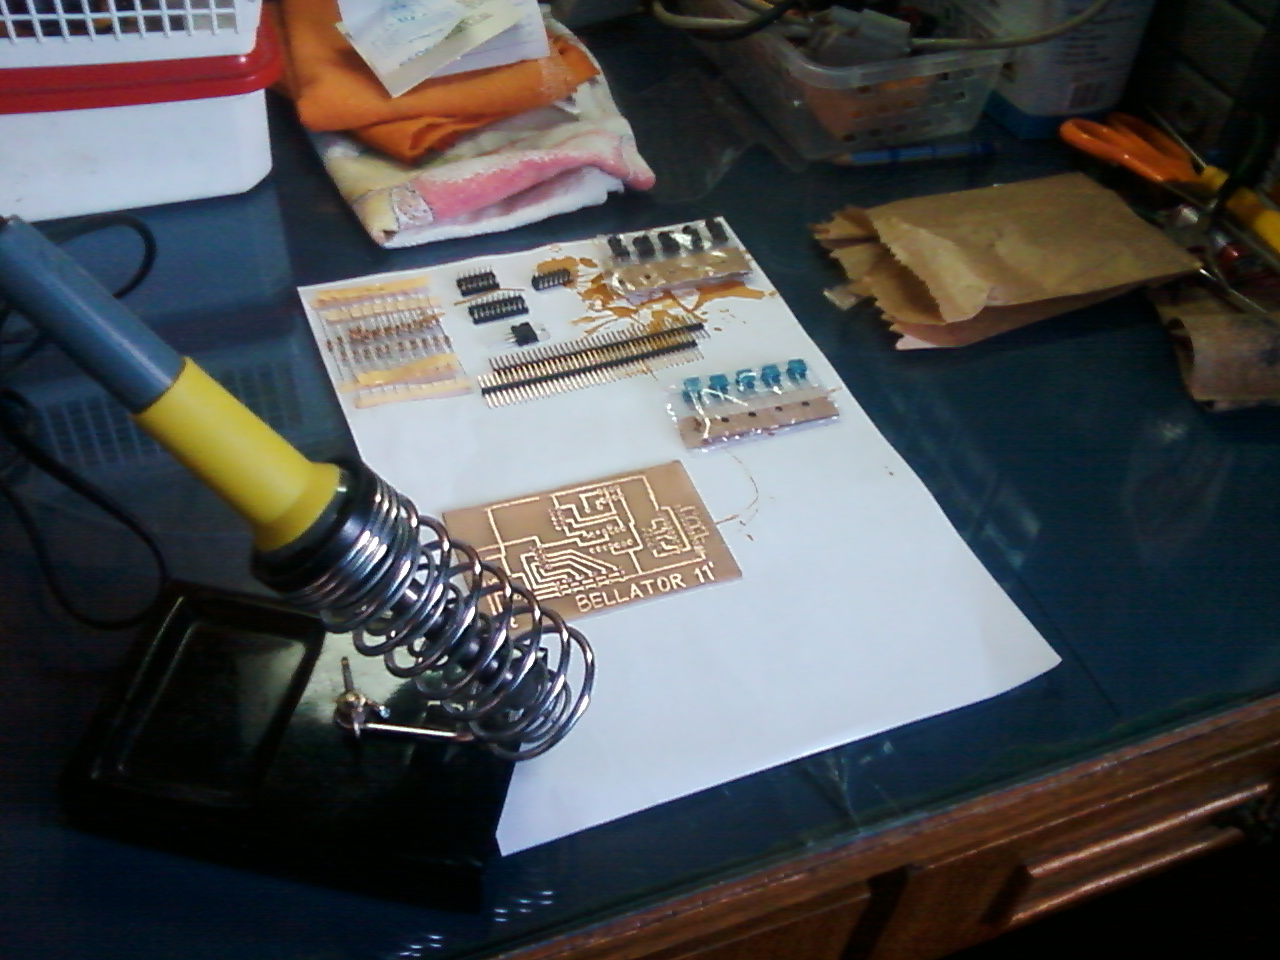
\includegraphics[width=0.8\textwidth]{./figs/placa-confeccao.jpg}
  \caption[Processo de confec��o da placa de roteamento.]
  {Processo de confec��o da placa de roteamento.}
  \label{fig:confeccao}
\end{figure}

%Descrever os fatores. Escrever requisitos. Descrever placa. Explicar a produ��o da placa. Por que usar o Eagle.

\subsection{Placa TS-7260}
\label{sec:ts}
%Descri��o do motivo da escolha da placa, implementa��o de c�digos auxiliares aos algoritmos (comunica��o, etc)...
Esta se��o explicar� como foi estruturado o software desenvolvido para a placa
TS-7260, cuja fun��o principal � realizar a interface entre o software do microcontrolador
C8051F340 e o algoritmo de navega��o (Fuzzy ou FCM).

\subsection{Configura��o da TS-7260}
O software da TS-7260 foi desenvolvido em C++, assim como os algoritmos de navega��o, a serem
explicados em detalhes na se��o~\ref{sec:algs}. A programa��o foi realizada em um computador comum.
Para realiza��o de testes na placa, o c�digo foi compilado para a TS-7260 atrav�s da utiliza��o de um
\emph{cross-compiler}, que pode ser baixado em~\cite{CC}. O arquivo bin�rio gerado pela compila��o
foi ent�o movido para uma pasta compartilhada na rede. Esta pasta foi disponibilizada atrav�s de um
servidor NFS (\emph{Network File System}) instalado no computador
onde o c�digo foi desenvolvido. A placa TS-7260 cont�m em um pendrive um linux compilado para a sua
arquitetura, que disponibiliza o cliente nfs, atrav�s do qual foi poss�vel montar a pasta compartilhada e rodar
o algoritmo. Posteriormente, para testes totalmente aut�nomos, o arquivo bin�rio foi copiado da pasta
compartilhada para o pendrive conectado � TS-7260, o que permite que o rob� execute a navega��o sem
necessidade de conex�o com o computador. O comando utilizado no terminal da TS-7260 para montar a pasta
compartilhada foi:

\begin{verbatim}
mount 192.168.0.3:/files /mnt
\end{verbatim}

onde \mbox{192.168.0.3} era o IP local da m�quina onde o software foi desenvolvido, \emph{/files}
o diret�rio compartilhado por rede e \emph{/mnt} a pasta onde deveria ser montado. Ap�s montar a pasta,
os seguintes comandos s�o executados:

\begin{verbatim}
cd /mnt
./tslogic fcm
\end{verbatim}
ou
\begin{verbatim}
./tslogic fuzzy
\end{verbatim}

Todas as configura��es da TS-7260 foram realizadas atrav�s de um terminal disponibilizado pela porta
serial. Atrav�s de um software como o HyperTerminal (Windows) ou o minicom (Linux) � poss�vel receber/enviar
dados. A placa TS-7260 possui tr�s portas de comunica��o serial, das quais duas foram utilizadas:
COM1 e COM2. A porta COM2 foi utilizada para conectar a TS-7260 ao microcontrolador C8051F340, para possibilitar
a troca de mensagens de comando com o microcontrolador (para alterar os n�veis de PWM dos motores), assim
como o recebimento das leituras dos sensores. A porta COM1, por sua vez, foi configurada para ser o terminal
mencionado anteriormente. Basta conectar um cabo serial da COM1 da TS-7260 ao computador para utiliz�-lo.
As configura��es da serial utilizadas foram (tanto COM1 quanto COM2): 115200 8N1, ou seja, \emph{baud-rate}
de 115200, caracteres de 8 (oito) bits, sem bit de paridade e com 1 (um) bit de parada. Atrav�s do terminal
disponibilizado na COM2, � poss�vel montar e acessar a pasta de rede compartilhada, conforme descrito no par�grafo
anterior.

\subsection{Software da TS-7260}
\label{sec:softwarets}
O c�digo que roda na TS-7260 � o que efetivamente controla o rob�. A parte principal do c�digo consiste
de um loop infinito, que executa os seguintes passos:

\begin{itemize}
	\item Envio de um SYNC para o microcontrolador: isto faz com que o microcontrolador responda
		um pacote com as leituras mais recentes dos sensores de dist�ncia, juntamente com as leituras
		dos encoders (esta comunica��o � realizada via porta serial);
	\item Leitura do pacote enviado pelo microcontrolador: recebe os dados do microcontrolador e
		utiliza os dados de convers�o dos sensores para acessar a tabela que mapeia
		o valor da convers�o para a dist�ncia em cent�metros, tabela esta que foi obtida conforme
		o procedimento especificado na se��o~\ref{sec:curvasensores}. Os valores de dist�ncia para
		cada sensor s�o ent�o armazenados, assim como as leituras dos encoders;
	\item Execu��o do algoritmo de navega��o: utiliza os dados armazenados para executar o algoritmo
		de navega��o, passando os valores de leitura dos sensores de dist�ncia. O algoritmo utiliza
		os dados para realizar a infer�ncia, retornando valores que indicam qual a��o o rob� deve tomar.
		O algoritmo de navega��o � executado tamb�m na placa TS-7260, mas n�o faz parte do mesmo software;
	\item Ajuste dos setpoints: nesta etapa, os dados retornados pelo algoritmo de navega��o s�o
		utilizados para o c�lculo do setpoint de cada roda (velocidade desejada), o setpoint � ent�o
		alterado de acordo;
	\item Ajuste de velocidade: esta etapa consiste do ajuste dos n�veis de PWM de cada roda, e utiliza
		para tal os valores de leitura dos encoders e o setpoint do passo anterior.
		O objetivo do ajuste de velocidade � fazer com que cada motor fique o mais pr�ximo poss�vel
		do setpoint estabelecido previamente. Este ajuste � apenas proporcional, simplesmente aumentando
		a velocidade caso a contagem do encoder esteja abaixo do setpoint ou diminuindo caso esteja
		acima;
	\item Envio das a��es: os n�veis de PWM definidos pelo ajuste de velocidade s�o enviados para
		o microcontrolador C8051F340, que efetiva a mudan�a.
\end{itemize}

O diagrama em blocos a seguir representa o funcionamento do software, demonstrando
tamb�m em que etapas ocorre a comunica��o com o microcontrolador e quando o algoritmo
de navega��o � executado. Vale lembrar que o algoritmo de navega��o (Fuzzy ou FCM) executa na placa
TS-7260 tamb�m, mas seu c�digo n�o faz parte do software da TS-7260 (tslogic), por este motivo est�
em um bloco separado no diagrama. As a��es descritas no bloco C8051F340 s�o executadas no
microcontrolador.

\tikzstyle{tsb} = [rectangle, draw=black!100, fill=blue!15!green!10,
    text width=8em, text centered, rounded corners, minimum height=1cm]
\tikzstyle{transition} = [rectangle, thick, draw=black!75, fill=black!20,
	minimum size=4mm]
\tikzstyle{line} = [draw, -latex']
\tikzstyle{8051b} = [rectangle, draw=black!100, fill=red!15, rounded corners,
	minimum height=1cm, text width=8em, text centered]
\tikzstyle{navb} = [rectangle, draw=black!100, fill=yellow!30, rounded corners,
	text width=8em, minimum height=1cm, text centered]
\tikzstyle{background} = [rectangle, fill=gray!50, inner sep=8mm, rounded corners=5mm]
	\tikzstyle{backgroundb} = [rectangle, fill=black!50, inner sep=2mm, rounded corners=5mm]

\begin{figure}[H]
	\centering
	\begin{tikzpicture}[node distance = 1.5cm, auto]
		% N�s e conex�es do diagrama
		\node [tsb] (opentty) {Configura serial};
		\node [tsb, below of=opentty] (sync) {Envia SYNC} edge [pre] (opentty);
		\node [tsb, below of=sync] (read) {Leitura do pacote} edge [pre] (sync);
		\node [tsb, below of=read] (alg) {Executa algoritmo de navega��o} edge [pre] (read);
		\node [navb, left=2cm of alg] (nrcv) {Recebe dados} edge [pre] (alg);
		\node [navb, below of=nrcv] (ninf) {Realiza a infer�ncia} edge [pre] (nrcv);
		\node [navb, below of=ninf] (nret) {Retorna as a��es} edge [pre] (ninf);
		\node [tsb, right=2cm of nret] (sadj) {Ajuste dos setpoints} edge [pre] (nret);
		\node [tsb, below of=sadj] (vadj) {Ajuste da velocidade} edge [pre] (sadj);
		\node [tsb, below of=vadj] (act) {Envia as a��es} edge [pre] (vadj);
		\node [tsb, below of=act] (end) {Loop} edge [pre] (act);
		\node [8051b, right=2cm of sync] (rcv) {Recebe SYNC} edge [pre, dashed] (sync);
		\node [8051b, below of=rcv] (spkg) {Envia pacote}
			edge [pre] (rcv)
			edge [post, dashed] (read);
		\node [8051b, right=2cm of act] (pwm) {Ajuste dos PWMs} edge [pre, dashed] (act);
		\path [line] (end) -- +(-2.5,0) |- (sync);
		% Background
		\begin{pgfonlayer}{background}
			\node [background, fit=(nrcv) (end) (opentty), label=above:TS-7260] {};
			\node [backgroundb, fit=(opentty) (end), label=below:tslogic] {};
			\node [backgroundb, fit=(nrcv) (nret), label=below:Fuzzy/FCM] {};
			\node [background, fit=(rcv) (pwm), label=above:C8051F340] {};
		\end{pgfonlayer}
	\end{tikzpicture}
	\caption[Diagrama em blocos software TS-7260]
	{Diagrama em blocos demonstrando o funcionamento do software da placa TS-7260.}
\end{figure}

\subsection{Considera��es}

Nesta se��o foram descritos os passos da equipe para alcan�ar o primeiro objetivo do projeto, a reconstru��o da plataforma rob�tica Bellator, tornando-a apta para utiliza��o no teste e compara��o de algoritmos de navega��o. Foram descritos os testes iniciais com o rob�, o projeto da nova placa de roteamento e a implementa��o do software da placa TS-7260.

\section{Algoritmos de Navega��o}
\label{sec:algs}
Esta se��o dedica-se � descri��o da implementa��o dos algoritmos de navega��o conforme descri��o te�rica dos mesmos apresentada na fundamenta��o te�rica. Mais espec�ficamente, ser�o descritos os c�digos respons�veis pela tomada de decis�es de ambos os algoritmos de navega��o que executam na placa TS-7260, o algoritmo de navega��o de l�gica Fuzzy cl�ssica, utilizando os mecanismos de infer�ncia propostos por \cite{MAMDAMI} e o ED-FCM, proposto por \cite{MENDONCA}.

\subsection{Algoritmo de Navega��o Fuzzy}
\label{sec:algfuzzy}
%Descri��o e referencia b�sica da biblioteca do fabro, adapta��o e utiliza��o. Descri��o das regras. INCOMPLETO
O algoritmo de Navega��o Fuzzy, baseado em infer�ncias sobre conjuntos Fuzzy, foi desenvolvido utilizando-se a biblioteca FLIE, desenvolvida originalmente pelo professor Jo�o Alberto Fabro~\cite{FABRO}. A FLIE, ou \emph{Fuzzy Logic Inference Engine}, � uma biblioteca que j� implementa um ambiente para a defini��o de conjuntos fuzzy e regras de infer�ncia sobre os mesmos, proporcionando � equipe mais tempo para o aprimoramento das regras e conjuntos e o teste dos mesmos. Este algoritmo ser� utilizado como base de compara��o para determina��o da efici�ncia do ED-FCM, descrito na se��o \ref{sec:algedfcm}. Nesta se��o, ser� descrito como a biblioteca FLIE foi utilizada neste projeto e como foram definidos os conjuntos fuzzy e as regras de infer�ncia, seguindo a fundamenta��o te�rica sobre o assunto apresentada na se��o \ref{sec:logfuzzy}.

\subsubsection{Vari�veis Lingu�sticas}
\label{sec:devarling}
A biblioteca FLIE, desenvolvida em C++ por J�ao Alberto Fabro, possui estruturas de dados, ou classes, prontas para serem utilizadas para defini��o de vari�veis lingu�sticas para bem como estruturas para a defini��o de regras de infer�ncia baseadas neste conjunto de vari�veis lingu�sticas, sendo apropriada para a elabora��o de um algoritmo de navega��o fuzzy. A biblioteca funciona de acordo com os princ�pios te�ricos fuzzy apresentados na se��o \ref{sec:logfuzzy}.

Para elaborar o controle fuzzy respons�vel pelo algoritmo de navega��o, � necess�rio, primeiramente, definir as vari�veis lingu�sticas e os conjuntos fuzzy associados �s mesmas. Em seguida, deve-se definir as vari�veis lingu�sticas de entrada e sa�da do sistema e as associar apropriadamente. Em seguida, � necess�rio definir o m�todo de defuzzifica��o e, finalmente, as regras de infer�ncia. Cada um destes passos ser� descrito em detalhes a seguir.

A biblioteca FLIE permite a defini��o de vari�veis lingu�sticas na classe \emph{linguisticvariable}, que pode ser composta por diversos conjuntos fuzzy, definidos a partir da classe \emph{category}. Cada \emph{category} � definida por uma faixa de valores v�lidos (\emph{range}), por 4 pontos que definem um trap�zio com os intervalos de subida, m�ximo e descida do n�vel de pertin�ncia do conjunto de entrada, para fuzzifica��o dos dados, e um nome apropriado, tal como Perto, Longe, R�pido, dependendo do contexto. Ou seja, cada valor de entrada � fuzzificado de acordo com seu n�vel de pertin�ncia a cada categoria (conjunto fuzzy) pertencente � vari�vel lingu�stica. A figura \ref{lingvar}, apresentada a seguir, demonstra de forma gr�fica esta estrutura.

\begin{figure}[H]
  \centering
  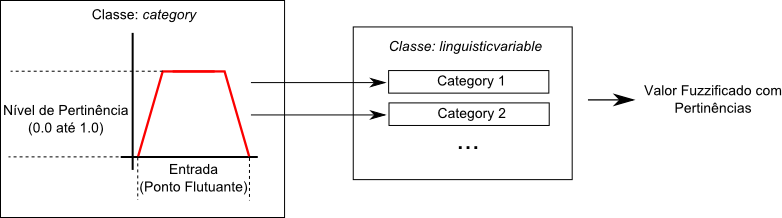
\includegraphics[width=0.8\textwidth]{./figs/lingvar.png}
  \caption[Estrutura de uma Vari�vel Lingu�stica no FLIE.]
  {Estrutura de uma Vari�vel Lingu�stica no FLIE.}
  \label{lingvar}
\end{figure}

Utilizando esta estrutura, foram desenvolvidas tr�s vari�veis lingu�sticas para a entrada do sistema e duas vari�veis lingu�sticas para a sa�da do sistema. Deve-se observar que foram definidas apenas tr�s vari�veis lingu�sticas de entrada por dois motivos: A biblioteca FLIE n�o aceita mais que tr�s entradas em uma regra de infer�ncia e um n�mero maior de entradas levaria � uma quantidade excessiva de regras de infer�ncia. As vari�veis lingu�sticas de entrada correspondem aos cinco sensores do rob�, sendo que o sensor frontal utiliza uma vari�vel lingu�stica, ``SensorFrente"~ e os dois pares de sensores laterais s�o agrupados em duas vari�veis lingu�sticas, ``SensorEsquerda"~ e ``SensorDireita"~ sendo que apenas o menor valor de leitura v�lida � selecionado nos pares de sensores laterais para ser fuzzificado. Cada uma destas vari�veis lingu�sticas est� definida com tr�s conjuntos fuzzy, totalizando nove conjuntos fuzzy organizados de acordo com a tabela \ref{tab:varsfuzzy}.

\begin{table}[H]
\centering
\begin{tabular}{|l|l|l|}
  \hline
  % after \\: \hline or \cline{col1-col2} \cline{col3-col4} ...
  \textbf{Vari�vel Lingu�stica} & \textbf{Conjunto Fuzzy} & \textbf{Fun��o de Pertin�ncia} \\
  \hline
  SensorEsquerda & PertoEsquerda & p(d) \\
  SensorEsquerda & MedioEsquerda & m(d) \\
  SensorEsquerda & LongeEsquerda & l(d) \\
  SensorFrente & Perto & p(d) \\
  SensorFrente & Medio & m(d) \\
  SensorFrente & Longe & l(d) \\
  SensorDireita & PertoDireita & p(d) \\
  SensorDireita & MedioDireita & m(d) \\
  SensorDireita & LongeDireita & l(d) \\
  \hline
\end{tabular}
\caption[Fun��es de Pertin�ncia e Conjuntos Fuzzy dos Sensores]{Fun��es de Pertin�ncia e Conjuntos Fuzzy dos Sensores.}
\label{tab:varsfuzzy}
\end{table}
As fun��es de pertin�ncia p(d), m(d), l(d), correspondentes a perto, m�dio e longe, s�o definitas pelos trap�zios da figura \ref{fuzzygraph_des}:

\begin{figure}[H]
  \centering
  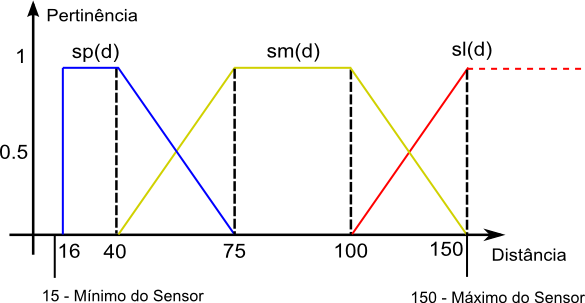
\includegraphics[width=0.8\textwidth]{./figs/fuzzygraph_des.png}
  \caption[Defini��o das Fun��es de Pertin�ncia perto, m�dio e longe.]
  {Defini��o das Fun��es de Pertin�ncia perto, m�dio e longe.}
  \label{fuzzygraph_des}
\end{figure}

Embora as fun��o de pertin�ncia sejam a mesma para os conjuntos fuzzy representando perto, m�dio e longe para as tr�s vari�veis lingu�sticas, cada vari�vel lingu�stica necessita de objetos da classe \emph{category} exclusivos e �nicos, por uma restri��o da biblioteca flie, e n�o � poss�vel utilizar o mesmo conjunto fuzzy para duas ou mais vari�veis lingu�sticas diferentes.

De forma an�loga, as vari�veis lingu�sticas de sa�da do sistema s�o definidas pelas vari�veis lingu�sticas ``Velocidade Motor"~ e ``Dire��o", representando a velocidade e a dire��o do deslocamento do rob�. Os conjuntos fuzzy associados � vari�vel lingu�stica Velocidade Motor foram definidos de forma a distribuir igualmente as faixas de PWM de 0 a 100\% da capacidade do motor em tr�s categorias: Lento, M�dio e R�pido. As fun��es de pertin�ncia que definem estes conjuntos fuzzy s�o l(p), m(p), r(p), onde p � a percentagem do PWM. Pode-se visualizar estas fun��es na figura \ref{defuzzygraph_velmotor}.

\begin{figure}[H]
  \centering
  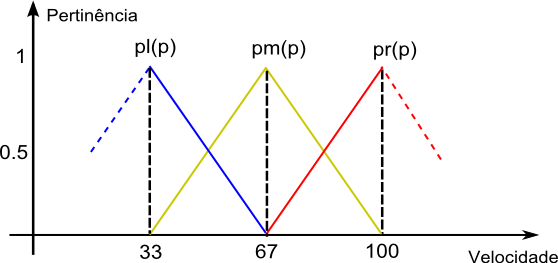
\includegraphics[width=0.8\textwidth]{./figs/defuzzygraph_velmotor.png}
  \caption[Defini��o das Fun��es de Pertin�ncia lento, m�dio e r�pido.]
  {Defini��o das Fun��es de Pertin�ncia lento, m�dio e r�pido.}
  \label{defuzzygraph_velmotor}
\end{figure}

Similarmente, foram definidos 5 conjuntos fuzzy para a vari�vel lingu�stica ``Dire��o": ViraEsquerda, ViraPoucoEsquerda, Reto, ViraPoucoDireita, ViraDireita, distribuindo igualmente entre estas classes todas as possibilidades de dire��o, desde virar totalmente para a esquerda (0�) at� totalmente para direita(180�), sendo que 90� representa movimento sem altera��o de dire��o. As fun��es de pertin�ncia que definem estes conjuntos fuzzy s�o ve(a), vpe(a), r(a), vpd(a), vd(a). O gr�fico em \ref{defuzzygraph_ang} ilustra estas fun��es.

\begin{figure}[H]
  \centering
  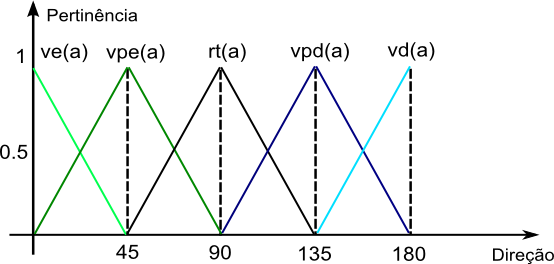
\includegraphics[width=0.8\textwidth]{./figs/defuzzygraph_ang.png}
  \caption[Defini��o das Fun��es de Pertin�ncia de Dire��o]
  {Defini��o das Fun��es de Pertin�ncia de Dire��o.}
  \label{defuzzygraph_ang}
\end{figure}


\subsubsection{Regras de Infer�ncia}

Ap�s definidas as vari�veis lingu�sticas, regras de infer�ncia podem ser elaboradas atrav�s da classe \emph{infrule}. Esta classe � composta de, no m�ximo, tr�s vari�veis lingu�sticas de entrada e uma vari�vel lingu�stica de sa�da, todas definidas pela classe \emph{linguisticvariable}, seguindo a estrutura na figura \ref{infrule}.

\begin{figure}[H]
  \centering
  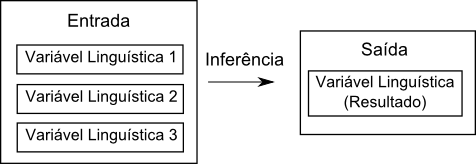
\includegraphics[width=0.8\textwidth]{./figs/infrule.png}
  \caption[Estrutura de uma regra de infer�ncia no FLIE.]
  {Estrutura de uma regra de infer�ncia no FLIE.}
  \label{infrule}
\end{figure}

Com as vari�veis lingu�sticas de entrada e sa�da pode-se criar regras de infer�ncia. Primeiramente, � necess�rio associar as vari�veis lingu�sticas que comp�e as regras de infer�ncia de entrada e sa�da � um objeto da classe \emph{fuzzy\_control}. Em seguida, cada regra � definida por uma sequ�ncia de valores fuzzy pertencentes �s vari�veis lingu�sticas de entrada e sa�da associadas com o objeto da classe \emph{fuzzy\_control}, sendo o �ltimo valor da sequ�ncia a sa�da fuzzy desejada para uma entrada correspondente aos um, dois ou tr�s valores antecedentes, que � o limite de entradas da biblioteca FLIE, como mencionado em \ref{sec:devarling}. Como deseja-se obter duas sa�das, uma para a velocidade e outra para a dire��o, foram necess�rios dois objetos desta classe, ambos com as mesmas entradas. Al�m disso, � necess�rio definir o m�todo de defuzzifica��o a ser utilizado pelo controle fuzzy. A equipe utilizou o m�todo da M�dia do M�ximo, descrito na se��o \ref{sec:fuzzycontrol}. Assim, as regras de infer�ncia seguem padr�o abaixo, de acordo com as vari�veis lingu�sticas definidas em \ref{sec:devarling}:
\begin{center}
SensorEsquerda, SensorFrente, SensorDireita, Velocidade Motor\\
SensorEsquerda, SensorFrente, SensorDireita, Dire��o
\end{center}

Em seguida, pode-se definir as regras atrav�s dos valores fuzzy v�lidos para cada vari�vel lingu�stica associada aos objetos \emph{fuzzy\_control}. A defini��o das regras � bastante intuitiva, emp�rica e altamente dependente da aplica��o. A equipe optou por definir um conjunto de regras arbitr�rio, realizar testes e, analisando os resultados preliminares, aprimorar o conjunto de regras. A tabela \ref{tab:regrasinf} representa o conjunto definitivo de 27 regras elaboradas pela equipe, que correspondem a todas as combina��es poss�veis de entradas para o controle fuzzy.

\begin{table}[H]
\centering
\label{tab:regrasinf}
\caption[Regras de Infer�ncia - Algoritmo Fuzzy]{Regras de Infer�ncia - Algoritmo Fuzzy.}
\begin{tabular}{|l|l|l|l|l|}
\hline
\textbf{SensorEsquerda} & \textbf{SensorFrente} & \textbf{SensorDireita} & \textbf{VelocidadeMotor} & \textbf{Dire��o} \\
\hline
PertoEsquerda & Perto & PertoDireita & Lento & ViraDireita \\
PertoEsquerda & Perto & MedioDireita & Lento & ViraDireita \\
PertoEsquerda & Perto & LongeDireita & Lento & ViraDireita \\
PertoEsquerda & Medio & PertoDireita & Lento & Reto \\
PertoEsquerda & Medio & MedioDireita & Lento & ViraDireita \\
PertoEsquerda & Medio & LongeDireita & Lento & ViraPoucoDireita \\
PertoEsquerda & Longe & PertoDireita & Medio & Reto \\
PertoEsquerda & Longe & MedioDireita & Lento & ViraPoucoDireita \\
PertoEsquerda & Longe & LongeDireita & Lento & ViraDireita \\
MedioEsquerda & Perto & PertoDireita & Lento & ViraEsquerda \\
MedioEsquerda & Perto & MedioDireita & Lento & ViraDireita \\
MedioEsquerda & Perto & LongeDireita & Lento & ViraPoucoDireita \\
MedioEsquerda & Medio & PertoDireita & Lento & ViraEsquerda \\
MedioEsquerda & Medio & MedioDireita & Medio & Reto \\
MedioEsquerda & Medio & LongeDireita & Medio & Reto \\
MedioEsquerda & Longe & PertoDireita & Lento & ViraPoucoEsquerda \\
MedioEsquerda & Longe & MedioDireita & Rapido & Reto \\
MedioEsquerda & Longe & LongeDireita & Medio & Reto \\
LongeEsquerda & Perto & PertoDireita & Lento & ViraEsquerda \\
LongeEsquerda & Perto & MedioDireita & Lento & ViraPoucoEsquerda \\
LongeEsquerda & Perto & LongeDireita & Lento & ViraDireita \\
LongeEsquerda & Medio & PertoDireita & Lento & ViraPoucoEsquerda \\
LongeEsquerda & Medio & MedioDireita & Medio & Reto \\
LongeEsquerda & Medio & LongeDireita & Rapido & ViraDireita \\
LongeEsquerda & Longe & PertoDireita & Lento & ViraEsquerda \\
LongeEsquerda & Longe & MedioDireita & Medio & Reto \\
LongeEsquerda & Longe & LongeDireita & Rapido & Reto \\
\hline
\end{tabular}
\end{table}

Finalmente, as regras definidas podem ser utilizadas para realizar as infer�ncias. A bilioteca FLIE recebe os dados de entrada n�o fuzzificados, os fuzzifica, atribuindo valores de pertin�ncia para cada categoria definida pelo desenvolvedor e determina o n�vel de ativa��o de cada regra de infer�ncia definida. Ap�s esta etapa, a FLIE defuzzifica o resultado seguindo o modelo de defuzzifica��o escolhido e retorna o resultado final, que pode ser utilizado para controlar a navega��o do rob�.

\subsubsection{Considera��es}

O algoritmo fuzzy produziu o comportamento adequado em navega��o rob�tica permitindo que o rob� fosse capaz de desviar obst�culos posicionados � direita, � esquerda e � frente do mesmo. Conforme foi descrito na se��o de testes, se��o \ref{sec:testes}, esse algoritmo possibilitou o rob� a navegar de forma aut�noma recebendo como entrada as leituras dos sensores. A vers�o descrita nessa se��o foi produzida ap�s a execu��o e conclus�o dos testes iniciais e avan�ados, se��es \ref{sec:testesini} e \ref{sec:testesavan}, respectivamente. Durante esses testes, o algoritmo foi submetido a uma s�rie de experimentos visando detectar erros de navega��o, isolar e corrig�-los. Esse processo foi realizado repetidas vezes e as fun��es de pertin�ncia e regras fuzzy foram aprimorados gradualmente. A tabela de fun��es, tabela \ref{tab:varsfuzzy}, e a tabela de regras, tabela \ref{tab:regrasinf}, representa a vers�o utilizada nos testes comparativos, descritos na se��o \ref{sec:testescomp}, que foi utilizada para obten��o do resultado final. 

\subsection{Algoritmo de Navega��o Baseado em FCM}
\label{sec:algedfcm}
%Descri��o da adapta��o do c�digo matlab, utiliza��o, conceitos.
Esta se��o tem por objetivo descrever o projeto e a implementa��o do algoritmo de navega��o baseado na abordage FCM, apresentada na se��o \ref{sec:fcm} da fundamenta��o te�rica. O projeto consistiu na defini��o dos conceitos de entrada, n�vel e sa�da, rela��es causais e respectivos pesos. A implementa��o foi desenvolvida em linguagem C++ e compilada para ser executada na placa TS-7260.

A id�ia do algoritmo foi controlar a dire��o do rob� ajustando a pot�ncia aplicada em cada roda, de forma independente, sendo que esta pode ser aplicada para a roda girar em ambos os sentidos. As seguintes hip�teses foram elaboradas para projetar o algoritmo:

\begin{enumerate}
\item Quando o rob� detectar um objeto � esquerda, aquele deve desviar para a direita;
\item Quando o rob� detectar um objeto � direita, aquele deve desviar para a esquerda;
\item Quando o rob� n�o detectar objetos nas laterais, este deve seguir em frente.
\end{enumerate}

Os movimentos ``desviar para a direita", ``desviar para a esquerda"~ e ``seguir em frente"~ podem ser obtidos controlando-se a pot�ncia e o sentido aplicado em cada roda. Desse modo, duas hip�teses foram imaginadas: as duas rodas girando para frente e as duas rotas girando em sentidos opostos. Os movimentos produzidos na primeira situa��o s�o:

\begin{enumerate}
\item Quando a roda direita girar mais r�pido que a roda esquerda, a mudan�a de dire��o � ``desviar para a esquerda";
\item Quando a roda esquerda girar mais r�pido que a roda direita, a mudan�a de dire��o � ``desviar para a direita";
\item Quando a roda esquerda girar na mesma intensidade que a roda direita, o movimento � ``seguir em frente".
\end{enumerate}

Os movimentos produzidos na segunda situa��o s�o:
\begin{enumerate}
\item Quando a roda direita girar para frente e a roda esquerda girar para tr�s, o movimento � ``desviar para a esquerda";
\item Quando a roda esquerda girar para frente e a roda direita girar para tr�s, o movimento � ``desviar para a direita".
\end{enumerate}

Desse modo, o algoritmo controla a dire��o do rob� calculando a ``intensidade de girar"~ a roda direita para tr�s ou para frente e a ``intensidade de girar"~ a roda esquerda para tr�s ou para frente, sendo que esse c�lculo recebe como entradas as dist�ncias registradas pelos sensores de dist�ncia na lateral direita, na frente e na lateral esquerda do rob�.

\subsubsection{Conceitos}
\label{subsec:conceitos}
Primeiramente, definiu-se a entrada do sistema de navega��o, a qual correspondeu �s leituras dos sensores de dist�ncia. Desse modo, foram criados tr�s conceitos de entrada:

\begin{enumerate}
\item SE - Representa a leitura do sensor lateral esquerdo;
\item SF - Representa a leitura do sensor frontal;
\item SD - Representa a leitura do sensor lateral direito.
\end{enumerate}

Esses conceitos guardam o valor da leitura da dist�ncia normalizada na faixa de 0 a 1, atrav�s da equa��o \ref{eq:normaliza}, sendo x o valor absoluto da dist�ncia (cm), MIN o valor m�nimo suportado pelo sensor e MAX o valor m�ximo.

\begin{equation}
\label{eq:normaliza}
y=\frac {x-MIN} {MAX-MIN}
\end{equation}

Em seguida, foram determinados os conceitos de n�vel do FCM, os quais estabelecem as infer�ncias resultantes dos valores dos conceitos de entrada. Foram definidos quatro conceitos de n�vel:

\begin{enumerate}
\item GDF - Representa a intensidade da decis�o de girar a roda direita para frente;
\item GDT - Representa a intensidade da decis�o de girar a roda direita para tr�s;
\item GEF - Representa a intensidade da decis�o de girar a roda esquerda para frente;
\item GET - Representa a intensidade da decis�o de girar a roda esquerda para tr�s.
\end{enumerate}

Os n�veis desses conceitos s�o ativados atrav�s de uma fun��o sigmoidal dependente dos valores dos conceitos de entrada. As equa��es \ref{eq:sig_frente} e \ref{eq:sig_tras} foram adaptadas da equa��o \ref{sigmoide}, apresentada na fundamenta��o te�rica, e operam em dom�nio (0, 1) e imagem (0, 1).

\begin{equation}
\label{eq:sig_frente}
f_1(x)=\frac{1} {1+e^{(-10x+4,5)}}
\end{equation}

\begin{equation}
\label{eq:sig_tras}
f_2(x)=1-\frac{1} {1+e^{(-10x+4,5)}}
\end{equation}

Por fim, definiu-se a sa�da do sistema de navega��o, a qual s�o os n�veis percentuais de pot�ncia de cada roda. Esse n�vel varia na faixa de -100\% a +100\% e o sinal indica o sentido de giro, sendo o sinal positivo  ``girar para frente"~ e o sinal negativo ``girar para tr�s"~. Desse modo, foram estabelecidos dois conceitos de sa�da:

\begin{enumerate}
\item RD Out - Representa o n�vel percentual de pot�ncia da roda direita;
\item RE Out - Representa o n�vel percentual de pot�ncia da roda esquerda.
\end{enumerate}

\subsubsection{Rela��es Causais}
\label{subsec:rel-causal}
Os conceitos foram interligados atrav�s das rela��es causais ilustradas na figura \ref{fig:fcm-proposto}. Esse FCM conecta os conceitos de entrada SD, SF e SE, atrav�s dos conceitos de n�vel GDF, GDT, GEF e GET, aos conceitos de sa�da RD Out e RE Out.

\begin{figure}[!htb]
	\centering
	\begin{tikzpicture}[node distance=1.3cm,>=stealth',bend angle=45,auto]

		\tikzstyle{place}=[circle,thick,draw=black!75,fill=blue!30,minimum size=6mm]
		\tikzstyle{red place}=[place,draw=red!75,fill=red!20]
		\tikzstyle{transition}=[rectangle,thick,draw=black!75,
			fill=black!20,minimum size=4mm]

		\tikzstyle{every label}=[red]
		\tikzstyle{weight}=[rectangle,draw=black!75,minimum size=5mm]

		\node [place, fill=red!30] (SE) {SE};
		\node [place, below=1cm of SE] (SF) {SF};
		\node [place, fill=green!30, below=1cm of SF] (SD) {SD};
		\node [place, fill=orange!30, below right=.75cm and 4cm of SD] (GET) {GET};
		\node [place, fill=orange!30, above=1cm of GET] (GEF) {GEF};
		\node [place, fill=orange!30, right=2cm of GEF] (REO) {RE Out};
		\node [place, fill=yellow!30, above right=.75cm and 4cm of SE] (GDT) {GDT};
		\node [place, fill=yellow!30, below=1cm of GDT] (GDF) {GDF};
		\node [place, fill=yellow!30, right=2cm of GDF] (RDO) {RD Out};
		\node [weight, fill=blue!30, left=1cm of GEF] (w9) {w9}
			edge [thick] (SF)
			edge [post,thick] (GEF);
		\node [weight, fill=green!30, below=.2cm of w9] (w2) {w2}
			edge [thick] (SD)
			edge [post,thick] (GEF);
		\node [weight, fill=green!30, left=1cm of GET] (w3) {w3}
			edge [thick] (SD)
			edge [post,thick] (GET);
		\node [weight, fill=red!30, above=.2cm of w9] (w4) {w4}
			edge [thick] (SE)
			edge [post,thick] (GEF);
		\node [weight, fill=red!30, left=1cm of GDT] (w6) {w6}
			edge [thick] (SE)
			edge [post,thick] (GDT);
		\node [weight, fill=blue!30, left=1cm of GDF] (w7) {w7}
			edge [thick] (SF)
			edge [post,thick] (GDF);
		\node [weight, fill=green!30, below=.2cm of w7] (w1) {w1}
			edge [thick] (SD)
			edge [post,thick] (GDF);
		\node [weight, fill=red!30, above=.2cm of w7] (w5) {w5}
			edge [thick] (SE)
			edge [post,thick] (GDF);
		\node [weight, fill=blue!30, below=.2cm of w6] (w8) {w8}
			edge [thick] (SF)
			edge [post,thick] (GDT);
		\node [weight, fill=blue!30, above=.2cm of w3] (w10) {w10}
			edge [thick] (SF)
			edge [post,thick] (GET);
		\node [weight, fill=yellow!30, left=.5cm of RDO] (w11) {w11}
			edge [thick] (GDF)
			edge [post,thick] (RDO);
		\node [weight, fill=yellow!30, above=.5cm of w11] (w12) {w12}
			edge [thick] (GDT)
			edge [post,thick] (RDO);
		\node [weight, fill=orange!30, left=.5cm of REO] (w13) {w13}
			edge [thick] (GEF)
			edge [post,thick] (REO);
		\node [weight, fill=orange!30, below=.5cm of w13] (w14) {w14}
			edge [thick] (GET)
			edge [post,thick] (REO);
	\end{tikzpicture}
	\caption[FCM proposto]{FCM proposto.}
	\fonte{Autoria pr�pria.}
	\label{fig:fcm-proposto}
\end{figure}

Para modificar o valor dos pesos em tempo de execu��o, introduziu-se ao sistema um conceito de estado que influencia os pesos de todas as rela��es causais. Os estados que o FCM proposto pode assumir s�o ``FRENTE"~ e ``TR�S", sendo que os pesos das rela��es causais quando o FCM estiver no primeiro estado est�o de acordo com a tabela \ref{tab:fcm-relacoes-frente} e os pesos no segundo estado, com a tabela \ref{tab:fcm-relacoes-tras}. O valor num�rico das intensidades das rela��es causais est�o de acordo com a tabela \ref{tab:pesos}.

\begin{table}[htb!]
	\centering
	\caption[Rela��es causais do controlador FCM proposto (Estado = FRENTE)]{Rela��es causais do controlador FCM proposto (Estado = FRENTE).}		
	\begin{tabular}[!htb]{ l l l l }
	  \hline
	  Rela��o causal & Descri��o & Efeito & Intensidade \\
	  \hline
		$w_1$ & SD influencia GDF & Positivo & Forte \\
		$w_2$ & SD influencia GEF & Positivo & Fraca \\
		$w_3$ & SD influencia GET & Positivo & M�dia \\
		
		$w_4$ & SE influencia GEF & Positivo & Forte \\
		$w_5$ & SE influencia GDF & Positivo & Fraca \\
		$w_6$ & SE influencia GDT & Positivo & M�dia \\
		
		$w_7$ & SF influencia GDF & Negativo & M�dia \\
		$w_8$ & SF influencia GDT & Positivo & Forte \\
		$w_9$ & SF influencia GEF & Negativo & M�dia \\
		$w_{10}$ & SF influencia GET & Positivo & Fraca \\
		
		$w_{11}$ & GDF influencia RD Out & Positivo & Forte \\
		$w_{12}$ & GDT influencia RD Out & Negativo & M�dia \\
		$w_{13}$ & GEF influencia RE Out & Positivo & Forte \\
		$w_{14}$ & GET influencia RE Out & Negativo & M�dia \\
	  \hline  	
	\end{tabular}
	\label{tab:fcm-relacoes-frente}
\end{table}

\begin{table}[htb!]
	\centering
	\caption[Rela��es causais do controlador FCM proposto (Estado = TR�S)]{Rela��es causais do controlador FCM proposto (Estado = TR�S).}		
	\begin{tabular}[!htb]{ l l l l }
	  \hline
	  Rela��o causal & Descri��o & Efeito & Intensidade \\
	  \hline
		$w_1$ & SD influencia GDF & Positivo & Fraca \\
		$w_2$ & SD influencia GEF & Positivo & Fraca \\
		$w_3$ & SD influencia GET & Positivo & Forte \\
		
		$w_4$ & SE influencia GEF & Positivo & Fraca \\
		$w_5$ & SE influencia GDF & Positivo & Fraca \\
		$w_6$ & SE influencia GDT & Positivo & Forte \\
		
		$w_7$ & SF influencia GDF & Negativo & Fraca \\
		$w_8$ & SF influencia GDT & Positivo & M�dia \\
		$w_9$ & SF influencia GEF & Negativo & M�dia \\
		$w_{10}$ & SF influencia GET & Positivo & Fraca \\
		
		$w_{11}$ & GDF influencia RD Out & Positivo & Fraca \\
		$w_{12}$ & GDT influencia RD Out & Negativo & Forte \\
		$w_{13}$ & GEF influencia RE Out & Positivo & Forte \\
		$w_{14}$ & GET influencia RE Out & Negativo & Fraca \\
	  \hline  	
	\end{tabular}
	\label{tab:fcm-relacoes-tras}
\end{table}

\begin{table}[htb!]
	\centering
	\caption[Valor num�rico dos pesos]{Valor num�rico dos pesos.}		
	\begin{tabular}[!htb]{ l l l l }
	  \hline
	  Intensidade & Valor num�rico \\
	  \hline
		FRACA & 0,125 \\
		M�DIA & 0,5 \\
		FORTE & 1,0 \\
	  \hline  	
	\end{tabular}
	\label{tab:pesos}
\end{table}

A transi��o de estado � feita atrav�s de uma regra ``SE-ENT�O"~, sendo que valor de L0 e L1 est�o de acordo com a tabela \ref{tab:limiar-values}.

\begin{itemize}
\item SE o conceito SF for menor que o limiar L0 e o estado for igual a FRENTE ENT�O o estado muda para TR�S.
\item SEN�O SE o conceito SF for maior que o limiar L1 e o estado for igual a TR�S ENT�O o estado muda para FRENTE.
\end{itemize}

\begin{table}[htb!]
	\centering
	\caption[Valor num�rico dos limiares L0 e L1]{Valor num�rico dos limiares L0 e L1.}		
	\begin{tabular}[!htb]{ l l l l }
	  \hline
	  Limiar & Valor num�rico \\
	  \hline
		L0 & 0,15 \\
		L1 & 0,25 \\
	  \hline  	
	\end{tabular}
	\label{tab:limiar-values}
\end{table}

\subsubsection{Ativa��o dos Conceitos}

As equa��es \ref{eq:gdf} a \ref{eq:get} determinam a ativa��o dos conceitos de n�vel GDF, GDT, GEF e GET, respectivamente. Essa ativa��o � gradual e herda a caracter�stica de suavidade das fun��es sigmoidais \ref{eq:sig_frente} e \ref{eq:sig_tras}. Os conceitos de sa�da $RD_{Out}$ e $RE_{Out}$ s�o uma m�dia ponderada entre os conceitos ``girar para frente"~ e ``girar para tr�s", aplicada �s rodas direita e esquerda, conforme as equa��es \ref{eq:rd_out} e \ref{eq:re_out}, respectivamente.

\begin{equation}
\label{eq:gdf}
GDF=\frac {w_1f_2(SD)+w_5f_1(SE)-w_7f_2(SF)} {w_1+w_5}
\end{equation}

\begin{equation}
\label{eq:gdt}
GDT=\frac {w_6f_2(SE)+w_8f_2(SF)} {w_6+w_8}
\end{equation}

\begin{equation}
\label{eq:gef}
GEF=\frac {w_4f_2(SE)+w_2f_1(SD)-w_9f_2(SF)} {w_4+w_2}
\end{equation}

\begin{equation}
\label{eq:get}
GET=\frac {w_3f_2(SD)+w_{10}f_2(SF)} {w_3+w_{10}}
\end{equation}

\begin{equation}
\label{eq:rd_out}
RD_{Out}=100 \times \frac {w_{11}GDF-w_{12}GDT} {FORTE}
\end{equation}

\begin{equation}
\label{eq:re_out}
RD_{Out}=100 \times \frac {w_{13}GEF-w_{14}GET} {FORTE}
\end{equation}

\subsubsection{Considera��es}

O FCM projetado ofereceu a capacidade de o rob� desviar obst�culos posicionados � direita, � esquerda e � frente do mesmo. Conforme foi descrito na se��o de testes, se��o \ref{sec:testes}, esse algoritmo possibilitou o rob� a navegar de forma aut�noma recebendo como entrada as leituras dos sensores. Contudo, a vers�o final do FCM foi obtida ap�s diversos testes, nos quais erros de navega��o foram encontrados, isolados e corrigidos repetidas vezes. Nesse processo, os pesos das rela��es causais foram modificados at� chegarem aos valores das tabelas \ref{tab:fcm-relacoes-frente} e \ref{tab:fcm-relacoes-tras}. A necessidade de implementa��o de um FCM com evento surgiu durante a execu��o de um experimento dos testes avan�ados, como � descrito na se��o \ref{sec:testesavan}. O evento foi implementado para resolver especificamente aquele problema de indecis�o. Com isso, a vers�o final do projeto de FCM apresentada nessa se��o foi capaz de resolver os problemas propostos nos experimentos dos testes comparativos, se��o \ref{sec:testescomp}, gerando resultados adequados para a compara��o com o algoritmo fuzzy, apresentado na se��o \ref{sec:algfuzzy}.

\section{Testes e An�lise de Resultados}
\label{sec:testes}

Esta se��o tem por objetivo apresentar a metodologia e elabora��o dos testes dos algoritmos de navega��o implementados pela equipe, utilizando-se de desenhos esquem�ticos e descri��o detalhada dos objetivos de cada teste, al�m das altera��es e ajustes aos par�metros e conceitos dos algoritmos realizados a partir dos resultados dos testes. Nesta se��o tamb�m � apresentada a an�lise e compara��o do comportamento de ambos os algoritmos de navega��o a partir dos resultados dos experimentos para cada algoritmo, ap�s submetidos �s mesmas condi��es de teste.

\subsection{Elabora��o dos Testes}

A metodologia de elabora��o dos testes da equipe visou possibilitar testes de sistema, verificando a funcionalidade b�sica dos algoritmos,  testes de comportamento visando eliminar erros de desenvolvimento e comportamentos indesejados para ambos os algoritmos e, finalmente, comparar o comportamento dos algoritmos submetidos �s mesmas condi��es iniciais de teste. Ao longo dos testes, v�rias altera��es foram realizadas tanto aos conjuntos \emph{fuzzy} e regras de infer�ncia do algoritmo de navega��o \emph{fuzzy} quanto aos conceitos e fun��es sigm�ides do algoritmo baseado em ED-FCM, antes de atingir a configura��o final descrita nas se��es \ref{sec:algfuzzy} e \ref{sec:algedfcm}.

Assim sendo, foram desenvolvidas tr�s principais etapas de testes:
\begin{enumerate}
    \item Testes Iniciais: Teste b�sico dos algoritmos visando observar a movimenta��o b�sica, sincronia das rodas e ajuste de par�metros.
    \item Testes Avan�ados: Testes realizados com mais obst�culos para avaliar a capacidade dos algoritmos em evitar colis�es com obst�culos.
    \item Testes Comparativos: Testes finais visando a compara��o do comportamento entre os algoritmos em diversas situa��es
\end{enumerate}

Tanto os testes iniciais quanto os avan�ados s�o essenciais para proporcionar uma an�lise de resultados confi�vel entre os algoritmos. Nas se��es seguintes, para cada teste desenvolvido, s�o apresentados diagramas esquem�ticos espaciais, representando a disposi��o dos obst�culos e a posi��o inicial do rob�, o comportamento apresentado pelo rob�, poss�veis altera��es e ajustes realizados nos algoritmos por conta dos resultados do teste.

\subsection{Testes Iniciais}
\label{sec:testesini}

%corredor interno e externo dainf
Foram elaborados dois testes iniciais, o primeiro visando observar o deslocamento simples e detec��o de um obst�culo simples pr�ximo a parede em um corredor (Figura \ref{algtest1}), e o segundo teste foi constru�do em um corredor mais largo que o primeiro, com alguns obst�culos obstruindo a passagem, definindo apenas um caminho poss�vel entre os obst�culos (figura \ref{algtest2}).

\begin{figure}[H]
  \centering
  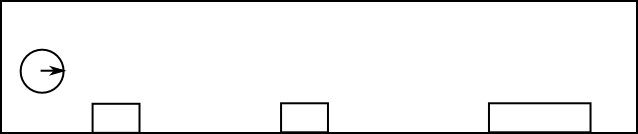
\includegraphics[width=0.8\textwidth]{./figs/algtest1.png}
  \caption[Configura��o do primeiro teste inicial.]
  {Configura��o do primeiro teste inicial.}
  \label{algtest1}
  \fonte{Autoria pr�pria}
\end{figure}

Ambos os algoritmos obtiveram resultados satisfat�rios, sendo capazes de realizar o percurso sem colidir com os obst�culos. Contudo, o algoritmo de navega��o \emph{fuzzy} mostrou-se excessivamente lento pr�ximo aos obst�culos. Concluiu-se que isto ocorreu devido ao valor m�ximo das fun��es de pertin�ncia ``Lento"~ e ``M�dio", serem muito baixos. A fun��o de pertin�ncia ``Lento"~ apresentava um valor m�ximo de apenas 20\% da velocidade m�xima e ``M�dio"~ correspondia a 50\%. A partir desta observa��o, as fun��es de pertin�ncia da velocidade foram alteradas para os novos valores, descritos na se��o \ref{sec:algfuzzy} de 33\% para ``Lento"~ e 66\% para ``M�dio". Ap�s os ajustes, o algoritmo mostrou-se mais r�pido no corredor, no mesmo teste.

\begin{figure}[H]
  \centering
  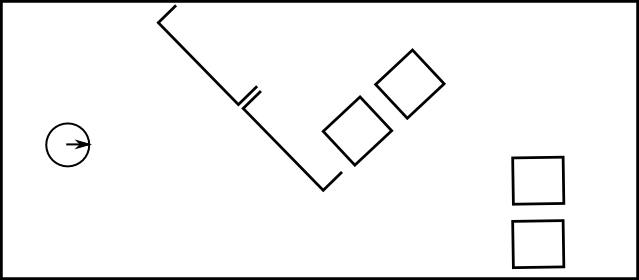
\includegraphics[width=0.8\textwidth]{./figs/algtest2.png}
  \caption[Configura��o do segundo teste inicial.]
  {Configura��o do segundo teste inicial.}
  \label{algtest2}
  \fonte{Autoria pr�pria}
\end{figure}

O segundo teste, ao contr�rio do primeiro, for�a os algoritmos a desviar de uma barreira imediatamente no caminho do rob� e encontrar a sa�da do corredor, logo ap�s a barreira, como ilustrado na figura \ref{algtest2}. Ao executar este teste pela primeira vez, o algoritmo \emph{Fuzzy} n�o foi capaz de fazer o desvio e encontrar a sa�da, devido a rea��o muito tardia e, ao mesmo tempo, muito forte. J� o algoritmo ED-FCM foi capaz de realizar o trajeto sem altera��es. A figura \ref{algtest2_caminho} apresenta o trajeto esperado, em verde, que � aproximadamente o mesmo que o realizado pelo algoritmo ED-FCM, e o trajeto percorrido pelo algoritmo \emph{Fuzzy} cl�ssico, em vermelho.

\begin{figure}[H]
  \centering
  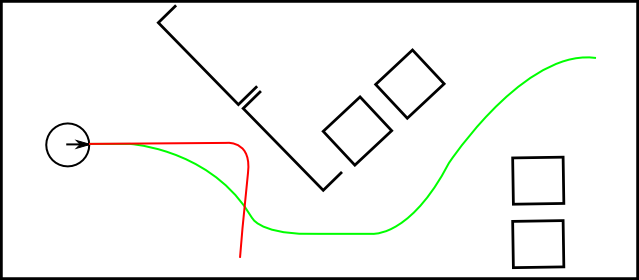
\includegraphics[width=0.8\textwidth]{./figs/algtest2_caminho.png}
  \caption[Caminho percorrido pelo algoritmo \emph{Fuzzy} (vermelho) e o caminho esperado (Verde).]
  {Caminhos percorridos no segundo teste inicial.}
  \label{algtest2_caminho} 
  \fonte{Autoria pr�pria}
\end{figure}

Para resolver este problema de rea��o tardia e tornar a navega��o do algoritmo \emph{Fuzzy} mais suave (em rela��o as curvas), a equipe aumentou a faixa de valores da fun��o de pertin�ncia da vari�vel lingu�stica perto, que era inicialmente 16 at� 25cm como dist�ncia de pertin�ncia m�xima e descida at� pertin�ncia nula na dist�ncia de 35 cent�metros para os valores finais apresentados na figura \ref{fuzzygraph_des}, fun��o p(d). Al�m disso, os conjuntos \emph{fuzzy} ``ViraPoucoEsquerda" e ``ViraPoucoDireita", inexistentes na primeira vers�o, foram adicionados e utilizados nas regras de infer�ncia da forma como foi apresentado na tabela \ref{tab:regrasinf}, visando iniciar a rea��o do rob� aos obst�culos mais cedo. Estas altera��es fizeram com que o algoritmo \emph{Fuzzy} cl�ssico realizasse o trajeto esperado, ap�s novo teste no mesmo ambiente.

\subsection{Testes Avan�ados}
\label{sec:testesavan}
%Corredor largo e estreito C300

Os testes avan�ados desenvolvidos pela equipe visam observar e otimizar o comportamento dos algoritmos, ou seja, al�m da simples capacidade de desvio de obst�culos, observar as escolhas realizadas pelos algoritmos em ambientes com mais de uma possibilidade de navega��o al�m da velocidade e agilidade do rob� nestes ambientes, com aten��o especial a situa��es espec�ficas que podem levar o rob� a ``travar"~e parar de navegar.

A equipe montou duas situa��es distintas para cumprir estes objetivos: O primeiro em um corredor similar ao segundo teste inicial, por�m mais longo e com mais obst�culos dispersos e o segundo em um corredor largo com obst�culos dispersos, provendo um ambiente aberto e imprevis�vel ao rob�.

\begin{figure}[H]
  \centering
  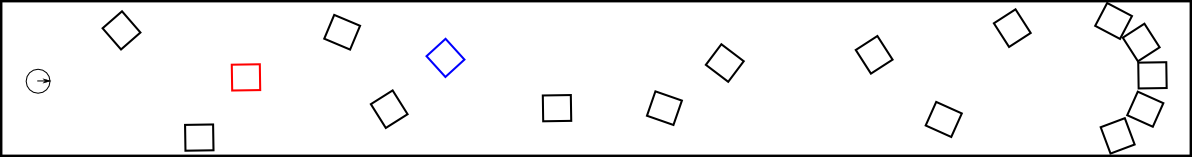
\includegraphics[width=0.8\textwidth]{./figs/algtestavancado_corredor.png}
  \caption[Ilustra��o do primeiro teste avan�ado.]
  {Ilustra��o do primeiro teste avan�ado.}
  \label{algtestavancado_corredor}
  \fonte {Autoria pr�pria}
\end{figure}

O algoritmo \emph{fuzzy} foi capaz de percorrer o primeiro teste avan�ado, ilustrado na figura \ref{algtestavancado_corredor}, retornando ao ponto de partida ap�s 5 minutos. Durante o percurso, houve apenas uma pequena colis�o com o obst�culo destacado em azul na figura acima. Neste experimento foi poss�vel observar lentid�o excessiva do rob� pr�ximo a obst�culos, levando a equipe a alterar a base de regras de infer�ncia levemente, de forma a reduzir o n�mero de regras que cont�m o conjunto \emph{fuzzy} ``Lento"~como sa�da de velocidade, acelerando a navega��o do rob� no mesmo teste. O conjunto de regras final, obtido ap�s as altera��es feitas a partir deste experimento, pode ser observado na tabela \ref{tab:regrasinf}. O algoritmo ED-FCM, em contrapartida, n�o foi capaz de percorrer o teste, apresentando indecis�o ao aproximar-se do obst�culo destacado em vermelho na figura \ref{algtestavancado_corredor}. Isto ocorreu devido � disponibilidade de espa�os iguais para o desvio deste obst�culo em ambas as op��es de desvio, o que anulou a intensidade de PWM em ambas as rodas. O efeito de anula��o � devido ao fato de as sigm�ides utilizadas na ativa��o dos conceitos serem sim�tricas, conforme as equa��es \ref{eq:sig_frente} e \ref{eq:sig_tras}. Desse modo, existe um ponto no qual a dist�ncia registrada pelos sensores laterais esquerdo e direito geram valores nos conceitos de entrada, SE e SD, que fazem com que os conceitos de n�vel GDF, GDT, GEF, GET (ver a explica��o desses conceitos na sec��o \ref{subsec:conceitos}) se igualem, ou seja, a tend�ncia de girar a roda para frente � igual a tend�ncia de girar a roda para tr�s, anulando, portanto, o PWM das rodas. Este problema foi corrigido atrav�s da implementa��o de um ``evento", espec�fico para aux�lio � navega��o nesta situa��o, que permitiu que o ED-FCM modificasse o peso das rela��es causais dinamicamente, conforme foi descrito na se��o \ref{subsec:rel-causal}. Essa modifica��o retirou do ED-FCM o comportamento sim�trico que resultava na anula��o dos PWMs e permitiu que o algoritmo resolvesse o problema de indecis�o, completando o percurso, sem novas indecis�es e travamentos, ap�s nova execu��o do experimento.

\begin{figure}[H]
  \centering
  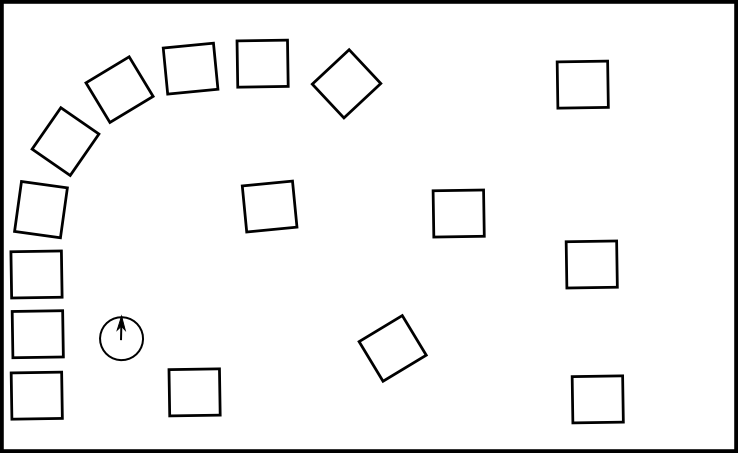
\includegraphics[width=1.0\textwidth]{./figs/algtestavancado_esparsos.png}
  \caption[Ilustra��o do segundo teste avan�ado.]
  {Ilustra��o do segundo teste avan�ado.}
  \label{algtestavancado_esparsos}
  \fonte{Autoria pr�pria}
\end{figure}

Ap�s todas as corre��es realizadas at� este ponto, a equipe elaborou um teste com diversos obst�culos esparsos e pontos de partida aleat�rios, visando detectar quaisquer problemas e comportamentos indesej�veis remanescentes nos algoritmos de navega��o. Em todas as execu��es dos algoritmos neste ambiente, representado na figura \ref{algtestavancado_esparsos}, o algoritmo foi capaz de navegar sem indecis�es e apenas raramente encostando em um obst�culo. Visto que n�o foi mais detectada a necessidade de corre��es e ajustes espec�ficos, este experimento permitiu concluir que os algoritmos estavam prontos para serem comparados em novos experimentos, descritos na se��o a seguir.

\subsection{Testes Comparativos}
\label{sec:testescomp}
%teste corredor "U" e teste FINAL
Os testes comparativos s�o, ap�s o desenvolvimento, corre��o e aprimoramento de ambos os algoritmos, a oportunidade de avaliar, de forma emp�rica, a nova abordagem de navega��o, proposta por Mendon�a, utilizando mapas cognitivos \emph{Fuzzy} em rela��o a uma abordagem utilizando um controle \emph{Fuzzy} cl�ssico. Foram elaborados dois experimentos visando expor ambos os algoritmos a diversos obst�culos e situa��es de indecis�o, possibilitando assim observar qual dos algoritmos responde melhor a estas situa��es. Os resultados de ambos os experimentos ser�o analisados de forma detalhada, visando determinar as principais caracter�sticas que diferenciam os algoritmos e justificar o comportamento observado.

\begin{figure}[H]
  \centering
  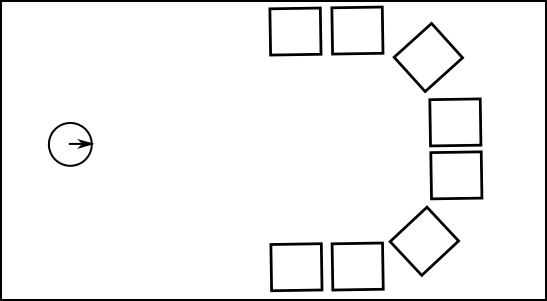
\includegraphics[width=0.8\textwidth]{./figs/algtestU.png}
  \caption[Ilustra��o do corredor sem sa�da.]
  {Ilustra��o do corredor sem sa�da.}
  \label{algtestU}
  \fonte{Autoria pr�pria}
\end{figure}

O primeiro teste comparativo consiste de um corredor sem sa�da, observ�vel na figura \ref{algtestU}, visando comparar o comportamento de ambos os algoritmos em uma situa��o comum de indecis�o, na qual s� � poss�vel sair atrav�s do mesmo caminho de entrada no corredor. Caso o algoritmo n�o seja capaz de detectar esta situa��o, poder� ficar preso.
Neste experimento, ambos os algoritmos de navega��o foram capazes de realizar o retorno e sair do corredor. O algoritmo \emph{Fuzzy} cl�ssico entrou no corredor no centro do mesmo, realizou um giro de 180� aproximadamente e saiu do corredor em um total de 26 segundos, enquanto que o algoritmo baseado em ED-FCM realizou pequenas convers�es ao longo da borda do corredor antes de encontrar a sa�da, o que levou cerca de 48 segundos. O caminho aproximado percorrido por ambos algoritmos pode ser visualizado no esbo�o da figura \ref{algtestU_caminhos}, onde o caminho executado pelo algoritmo \emph{Fuzzy} est� em vermelho e o ED-FCM em azul.

\begin{figure}[H]
  \centering
  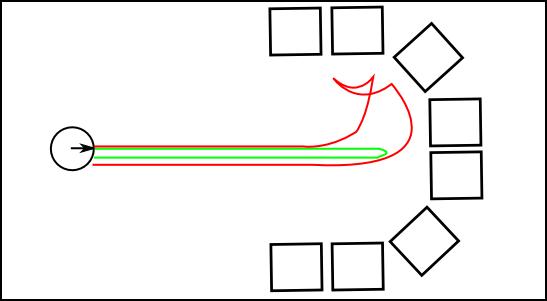
\includegraphics[width=0.8\textwidth]{./figs/algtestU_caminhos.png}
  \caption[Esbo�o do caminho percorrido pelo \emph{Fuzzy}(Vermelho) e ED-FCM(Azul).]
  {Esbo�o dos caminhos percorridos no primeiro teste comparativo.}
  \label{algtestU_caminhos}
  \fonte{Autoria pr�pria}
\end{figure}

Analisando este resultado, pode-se observar que o algoritmo \emph{Fuzzy} cl�ssico apresentou facilidade em retornar e sair do corredor. Isto deve-se � tend�ncia de virar para a direita quando a entrada do mecanismo de infer�ncia � ``Perto" para o sensor frontal e igual nos sensores laterais. Esta tend�ncia foi introduzida visando evitar a parada do rob� em situa��es similares a esta, e foi capaz de resolver esse experimento rapidamente, como esperado. As tr�s regras de infer�ncia respons�veis por esta tend�ncia, retiradas da tabela \ref{tab:regrasinf}, s�o:

\begin{center}
PertoEsquerda, Perto, PertoDireita $\implies$ Lento, ViraDireita \\
MedioEsquerda, Perto, MedioDireita $\implies$ Lento, ViraDireita \\
LongeEsquerda, Perto, LongeDireita $\implies$ Lento, ViraDireita
\end{center}

Em compensa��o, o algoritmo baseado em ED-FCM apresentou dificuldades nesta situa��o. Na figura \ref{algtestU_caminhos} � vis�vel que o algoritmo ED-FCM tratou inicialmente o corredor como um obst�culo, tentando desviar-se do mesmo pela esquerda. Ao detectar obst�culos em todos os sensores, o evento, implementado como solu��o do problema detectado no segundo teste avan�ado, descrito em \ref{sec:testesavan}, fazendo com que o rob� retorne e tente, novamente, fazer o desvio do obst�culo pela direita. Por�m, na segunda tentativa, � detectada maior disponibilidade de espa�o � direita do rob�, fazendo com que o mesmo contorne o corredor e encontre a sa�da.

\begin{figure}[H]
  \centering
  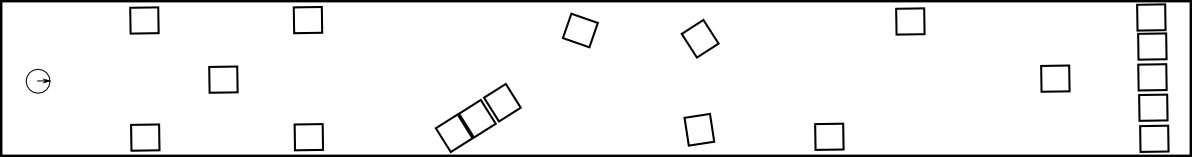
\includegraphics[width=0.8\textwidth]{./figs/algtestfinal.png}
  \caption[Esbo�o do segundo teste comparativo.]
  {Esbo�o do segundo teste comparativo.}
  \label{algtestfinal}
  \fonte{Autoria pr�pria}
\end{figure}

O segundo teste comparativo foi montado em um corredor longo, similarmente ao primeiro teste avan�ado, por�m com mais situa��es que possam causar indecis�es. Este teste possibilitou a observa��o da capacidade de decis�o, evas�o de obst�culos e tempo de ida e volta a partir do ponto de partida, vis�vel na figura acima, para ambos os algoritmos. O algoritmo \emph{fuzzy} foi capaz de percorrer o experimento em 4 minutos e 36 segundos, colidindo suavemente com um dos obst�culos, enquanto que o ED-FCM fez seu percurso em 4 minutos e 2 segundos, colidindo com dois obst�culos que compunham a parede do final do corredor enquanto tentava encontrar a sa�da do local. A figura abaixo mostra os caminhos percorridos por cada algoritmo, real�ando os obst�culos com os quais houve colis�o, sendo vermelho para o \emph{Fuzzy} cl�ssico e azul para o ED-FCM.

\begin{figure}[H]
  \centering
  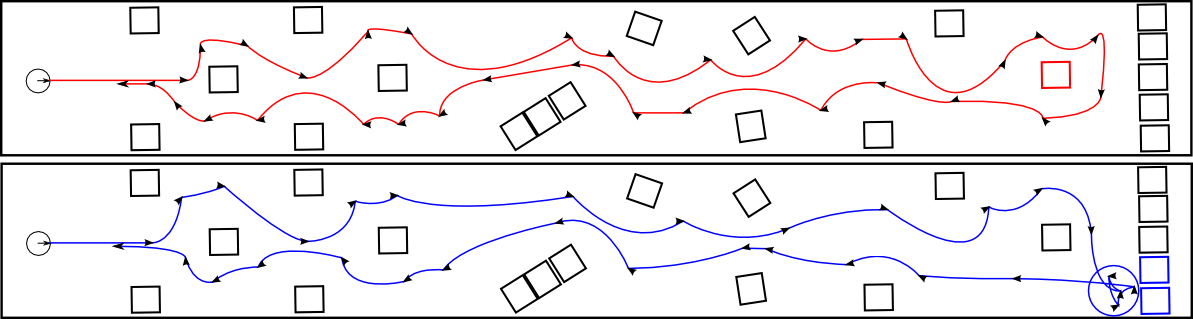
\includegraphics[width=1.0\textwidth]{./figs/algtestfinal_caminhos.png}
  \caption[Esbo�o do caminho percorrido pelo \emph{Fuzzy}(Vermelho) e ED-FCM(Azul).]
  {Esbo�o dos caminhos percorridos no primeiro teste comparativo.}
  \label{algtestfinal_caminhos}
  \fonte{Autoria pr�pria}
\end{figure}

Neste experimento foi not�vel a diferen�a de cerca de 14\% no tempo total levado pelo algoritmo \emph{fuzzy} para percorrer o experimento em rela��o ao algoritmo ED-FCM, apesar da colis�o com os obst�culos que demarcavam o final da �rea de testes e da dificuldade do algoritmo ED-FCM em encontrar a sa�da deste local, circulado em azul na figura \ref{algtestfinal_caminhos}. Esta dificuldade foi causada pela mesma situa��o encontrada pelo algoritmo no experimento anterior, no corredor sem sa�da. Ao tentar desviar do obst�culo pela esquerda, o algoritmo ED-FCM demorou cerca de 30 segundos para detectar a impossibilidade do desvio pela esquerda e voltar para o caminho correto. Se desconsiderarmos esta situa��o e os 30 segundos de atraso causados pela mesma, pode-se observar que o algoritmo ED-FCM percorreu o restante do experimento cerca de 23\% mais rapidamente que o algoritmo \emph{Fuzzy} cl�ssico, sem pausas prolongadas. O algoritmo \emph{Fuzzy}, apesar de ter colidido suavemente com um obst�culo, demarcado em vermelho na figura \ref{algtestfinal_caminhos}, mostrou-se mais cauteloso, n�o apresentando problemas durante o experimento como um todo. A colis�o pode ser explicada devido � tentativa de desviar da parede, que fez com que o obst�culo aparecesse subitamente nos sensores do rob�. Apenas o parafuso da roda encostou no obst�culo, deslocando a caixa em menos de 5 cent�metros.

De uma forma geral, o segundo teste comparativo possibilitou a equipe concluir que ambos os algoritmos de navega��o, apesar de algumas diferen�as no tratamento de situa��es espec�ficas e do tempo necess�rio para realizar o percurso, apresentaram resultados muito similares quanto � trajet�ria e decis�es tomadas ao longo do experimento.

\subsection{Considera��es}
Nesta se��o, foram apresentadas todas as etapas de elabora��o e execu��o dos testes, bem como todos os ajustes e corre��es dos algoritmos de navega��o desenvolvidos neste projeto. Tamb�m foram apresentados os testes comparativos, seus resultados e an�lise. Foi poss�vel observar que, com exce��o � situa��es espec�ficas, ambos os algoritmos apresentam comportamentos similares, embora o algoritmo baseado em ED-FCM apresente maior agressividade e o algoritmo \emph{Fuzzy} cl�ssico uma cautela maior pr�ximo a obst�culos. A partir destas informa��es, a equipe concluiu que nenhum dos algoritmos pode ser considerado como ``melhor" que o outro, por�m, existem diversas vantagens e desvantagens para cada um dos algoritmos, o que pode tornar um mais apropriado que o outro em determinadas situa��es. A lista a seguir mostra as vantagens e desvantagens observadas pela equipe:

\begin{enumerate}
\item Implementa��o: A implementa��o inicial do algoritmo \emph{Fuzzy} cl�ssico � mais complexa, exigindo a defini��o de diversos conjuntos \emph{Fuzzy}, vari�veis lingu�sticas e regras de infer�ncia, enquanto que o ED-FCM exige apenas a defini��o de conceitos, as rela��es causais entre eles e suas fun��es de ativa��o.
\item Altera��es: Ap�s a implementa��o inicial, o algoritmo \emph{Fuzzy} cl�ssico mostrou-se mais f�cil de alterar, quando necess�rio mudar o comportamento do algoritmo, enquanto que o ED-FCM � mais complexo de alterar, devido � dificuldade de determinar a quais conceitos e rela��es est�o produzindo o comportamento indesejado.
\item Comportamento: O algoritmo \emph{Fuzzy} apresenta maior cautela pr�ximo a obst�culos e maior facilidade de sair de situa��es com diversos obst�culos pr�ximos, enquanto que o ED-FCM apresenta dificuldade nestas situa��es, por�m maior agilidade em ambientes abertos e com menor n�mero de obst�culos dispersos.
\end{enumerate} 





\chapter{Conclus�o}

O presente trabalho de conclus�o de curso apresentou objetivos abrangentes, envolvendo desenvolvimento de hardware e software. No contexto da navega��o rob�tica, surgiu a necessidade de se utilizar um rob� real com a finalidade de se obter resultados mais significativos. Desse modo, foi elaborado um projeto cujo escopo tamb�m foi reconstruir e adequar uma plataforma rob�tica previamente dispon�vel, que � descrita na sec��o \ref{sec:estpro}, por�m que n�o estava em condi��es de uso imediato. A equipe procedeu com testes em laborat�rio de eletr�nica afim de avaliar as condi��es iniciais do rob�, conforme � descrito na sec��o \ref{sec:testecomp}. Uma an�lise de software foi efetuada e o c�digo original do microcontrolador C8051F340DK, disponibilizado como parte integrante do rob� Bellator \cite{BELLATOR}, foi avaliado e reconfigurado de acordo com as necessidades do projeto, o que � descrito em detalhes na se��o \ref{sec:codmicro}. Havendo necessidade de implementa��o de hardware, a equipe projetou e construiu uma placa de roteamento para alimentar os sensores e encoders, assim como tratar os sinais destes e os de PWM, como � descrito na se��o \ref{sec:desroteamento}. Finalmente, o hardware acoplado foi configurado e o software que executou os algortimos de navega��o foi desenvolvido, conforme a se��o \ref{sec:ts}. Com isso, a equipe concluiu a primeira parte do projeto, a qual consistiu na reconstru��o e adequa��o do rob� Bellator.

Estando a plataforma rob�tica funcional, seguiram-se o projeto e implementa��o dos algoritmos de navega��o propostos. A L�gica Fuzzy foi estudada e apresentada na se��o \ref{sec:logfuzzy} e a metodologia de Mapas Cognitivos Fuzzy (FCM) foi estudada e apresentada na se��o \ref{sec:fcm}. Com a teoria fundamentada, a equipe projetou os algoritmos e implementou-os na linguagem C++, compilados para executar no hardware acoplado, placa TS-7260. O projeto e a implementa��o dos algoritmos de navega��o Fuzzy e FCM s�o descritos em detalhes nas se��es \ref{sec:algfuzzy} e \ref{sec:algedfcm}, respectivamente. Ap�s a implementa��o, a equipe submeteu os algoritmos a uma s�rie de testes b�sicos, denominada Testes Iniciais, que serviram para fornecer a primeira realimenta��o do projeto dos algoritmos e pode ser lido na se��o \ref{sec:testesini}. Finalizados esses testes, foram elaborados testes complexos, denominados Testes Avan�ados, para estressar os sistemas de navega��o propostos e fornecer a segunda realimenta��o do projeto dos algoritmos, conforme � descri��o na se��o \ref{sec:testesavan}. Finalmente, ap�s os testes avan�ados, os algoritmos resolviam problemas complexos de navega��o, como o corredor sem sa�da e o problema de decis�o quando dois obst�culos laterais e um frontal era colocado diante do rob�, e poderiam ser usados nos testes finais, que forneceram os dados para a an�lise de resultados e foram denominados Testes Comparativos, conforme � descrito na se��o \ref{sec:testescomp}. Com isso foi conclu�do outros dois objetivos do projeto, que foram o projeto e implementa��o dos algoritmos de navega��o e a elabora��o e execu��o de uma metodologia de testes comparativos entre os algoritmos.

Para trabalhos futuros utilizando a plataforma Bellator reconstru�da, a equipe recomenda combinar sensores de ultra-som ao sensores infra vermelho, justificando isso porque os sensores de ultra-som apresentam uma faixa de opera��o cuja dist�ncia m�nima � menor que a do infra-vermelho, podendo capturar dist�ncias de 2 cm. Atualmente a dist�ncia m�nima suportada pelo sistema de navega��o � de 15 cm, com os sensores de ultra-som, os algoritmos poderiam operar em uma faixa mais abrangente. Outra sugest�o � introduzir ao sistema uma realimenta��o por b�ssola pois nesse projeto a realimenta��o odom�trica fornecida pelos encoders � utilizada para ajustar a velocidade das rodas e n�o faz uma interpreta��o da dire��o do rob�. Para tornar o rob� seguro para o manuseio, sugere-se a fixa��o dos sensores parafusando-os no chassi do Bellator e acoplando uma casca que proteja os circuitos microcontrolados. A equipe tamb�m recomenda a reconstru��o da placa de roteamento utilizando um m�todo industrial para confecc��o de placas de circuito impresso. Para os sistemas de navega��o, um trabalho futuro de grande riqueza seria introduzir ao sistema a capacidade de interpretar a posi��o do rob� em rela��o a um referencial. Com isso, o rob� seria capaz de resolver problemas nos quais este deve partir de um ponto inicial no espa�o a um ponto final, guiando-se pelos sensores para evitar colis�es e realimentar-se por um sistema de posicionamento para corrigir a traget�ria. Outro trabalho, produto deste, seria introduzir ao sistema uma mem�ria a qual pudesse mapear os obst�culos capturados pelos sensores do rob�, assim sendo, produzir-se-ia um artefato aut�nomo capaz de mapear terrenos. Outro aprimoramento da plataforma seria implementar um sistema de controle remoto por joystick, na qual uma base remota podesse pilotar o rob� via joystick. Finalmente, a equipe sugere um projeto futuro no qual seja implementado um sistema de vis�o computacional por c�mera de v�deo.

A equipe concluiu esta monografia justificando que os objetivos descritos na introdu��o, se��o \ref{rec:obj}, foram alcan�ados e est�o de acordo com os requisitos m�nimos de um curso de Engenharia de Computa��o. Os problemas encontrados na execu��o do projeto est�o associados ao escopo abrangente do mesmo, o qual envolveu o desenvolvimento de hardware e software em um projeto integrador. A subdivis�o do projeto em diversos objetivos, sendo um pr�-requisito para o outro, foi inevit�vel para alcan�ar os resultados finais. A equipe encontrou dificuldades durante a reconstru��o do rob�, configura��o da placa TS-7260, testes integrados de funcionamento do rob�, implementa��o dos algoritmos, execu��o dos testes dos algoritmos e an�lise de resultados. Durante a recontru��o, os componentes eletr�nicos foram testados isoladamente e houve riscos de haver danos, o que representaria atrasos no projeto. A placa TS-7260 apresentou complexidade para ser configurada pois n�o houve um t�cnico dispon�vel para auxiliar a equipe, a qual teve que aprender a trabalhar com esse hardware. Nos testes de integra��o da C8051F340DK e da TS-7260, que determinaram o funcionamento da plataforma rob�tica, foi exigido processos de depura��o integrados, nos quais os problemas foram isolados e corrigidos repetidas vezes. A implementa��o dos algoritmos at� a vers�o final, que foi utilizada nos testes comparativos, foi realizada paralelamente aos testes b�sicos e avan�ados, nas quais os problemas de navega��o foram detectados, isolados e corrigidos repetidas vezes. A metodologia de testes escolhida foi elaborada pela equipe e foram efetuados v�rios experimentos com registro em v�deo at� que se atingessem os resultados finais. Tendo com base os v�deos gravados e a experi�ncia em campo observada, a equipe precisou analisar os resultados, discut�-los e extrair conclus�es para finalizar o projeto, sendo que essa tarefa representou um trabalho cient�fico. 


%---------- Referencias ----------
\bibliography{reflatex} % geracao automatica das referencias a partir do arquivo reflatex.bib


%---------- Apendices (opcionais) ----------
\apendice
\chapter{Nome do Ap\^endice}

Use o comando {\ttfamily \textbackslash apendice} e depois comandos {\ttfamily \textbackslash chapter\{\}}
para gerar t\'itulos de ap\^en-dices.


% ---------- Anexos (opcionais) ----------
\anexo
\chapter{Nome do Anexo}

Use o comando {\ttfamily \textbackslash anexo} e depois comandos {\ttfamily \textbackslash chapter\{\}}
para gerar t\'itulos de anexos.

\end{document}

